% !TEX encoding = UTF-8 Unicode
% !TEX TS-program = xelatex
%%=================================================
%%
%% Department of Electrical and Computer Engineering
%% Project Report Template
%%
%% 1. "thesis.tex" - Only need to comment/uncomment parts that need compiled.
%%
%% 2. "info.tex" - Edit this file to define all your strings.
%%
%% 3. Edit these files for your report:
%%    1. abstract_th.tex       - บทคัดย่อ ภาษาไทย
%%    2. abstract_en.tex       - บทคัดย่อ ภาษาอังกฤษ
%%    3. ack_th.tex            - กิตติกรรมประกาศ ภาษาไทย
%%    4. ack_en.tex            - กิตติกรรมประกาศ ภาษาอังกฤษ (ไม่ได้ใช้)
%%    5. acronyms.tex          - คำย่อต่าง ๆ (ถ้ามี)
%%    6. chapter[1-5].tex      - รายงานแต่ละบท (บทที่ 1 - 5)
%%    7. refs.bib              - รายการเอกสารอ้างอิง
%%    8. appendix[A,B,...].tex - ภาคผนวก ก ข ...
%%
%%=================================================
\documentclass[12pt,a4paper,oneside]{book}
\newcommand{\mycomment}[1]{}

%%=================================================
%% START Packages
%%=================================================

%% Required packages for thesis layout (do not remove)
\usepackage{TUthesis}

%% Put everything else in "mystyle" package
\usepackage{mystyle}

%%=================================================
%% END Packages
%%=================================================


%%=================================================
%% START Project info
%%=================================================

%% Edit project information in the file "info.tex"
%%================================================
%% START Project info
%%================================================

%% Thesis for Master or Dissertation for PhD
\newcommand{\thesistype}{Thesis}

%% Thesis title in mixed case
\newcommand{\titleThai}{เว็บส่วนต่อประสานสำหรับการส่งงานเขียนโปรแกรมโดยใช้ Rest API}
\newcommand{\titleEng}{REST API for programming assignment with OPEN API}

%% Student name(s) i.e. author(s) of this thesis
%% Order suggestion: by alphabetical order
\newcommand{\authorAThai}{นางสาวดาราวิไล เชียงปวน}
\newcommand{\authorBThai}{นางสาว}
\newcommand{\authorAEng}{Ms. Darawilai Chiangpuan}
\newcommand{\authorBEng}{Ms.}


%% Degree that this thesis is for
\newcommand{\degreeThai}{วิศวกรรมศาสตรบัณฑิต}
\newcommand{\degreeEng}{Bachelor of Engineering}

%% Major
\newcommand{\majorThai}{วิศวกรรมคอมพิวเตอร์}
\newcommand{\majorEng}{Computer Engineering}

%% Date of submission
\newcommand{\submissionDayThai}{17}
\newcommand{\submissionDayEng}{17}
\newcommand{\submissionMonthThai}{กันยายน}
\newcommand{\submissionMonthEng}{September}
\newcommand{\submissionYearThai}{2564}
\newcommand{\submissionYearEng}{2021}

%% Academic year for thesis submission
\newcommand{\academicYearThai}{2564}
\newcommand{\academicYearEng}{2021}

%% Institute/department
\newcommand{\facultyThai}{คณะวิศวกรรมศาสตร์}
\newcommand{\facultyEng}{Faculty of Engineering}

%% keywords
\newcommand{\keywordThai}{ฟิชชิง การยืนยันเซิร์ฟเวอร์ การยืนยันผู้ใช้}
\newcommand{\keywordEng}{Phishing, server authentication, client authentication, certificates}

\newcommand{\headOfDepartmentThai}{ผู้ช่วยศาสตราจารย์ ดร. นพพร ลีปรีชานนท์}
\newcommand{\headOfDepartmentEng}{Asst. Dr. Nopporn Leepreechanont}
\newcommand{\advisorThai}{อาจารย์ นาวิน สมญาติ}
\newcommand{\advisorEng}{Prof. Nawin Somyat}

\newcommand{\committeeA}{อาจารย์ ดร. พิศาล แก้วประภา }
\newcommand{\committeeB}{อาจารย์ วชิรา พรหมสาขา ณ สกลนคร}
%\newcommand\dean{}
%%================================================
%% END Project info
%%================================================


%%=================================================
%% END Project info
%%=================================================

%%+++++++++++++++++++++++++++++++++++++++++++++++++
%% EDIT - Uncomment the type of report to compile
%%+++++++++++++++++++++++++++++++++++++++++++++++++
%\setReportType{Proposal}
%\setReportType{Proposal}
%\setReportType{Progress 1}
\setReportType{Progress 2}
%\setReportType{Final}

%%+++++++++++++++++++++++++++++++++++++++++++++++++
%% EDIT - Uncomment this line if you have acronyms page
%%+++++++++++++++++++++++++++++++++++++++++++++++++
\addAcronyms{true}

%%+++++++++++++++++++++++++++++++++++++++++++++++++
%% EDIT - Uncomment this line if you have listings page
%%+++++++++++++++++++++++++++++++++++++++++++++++++
\addListOfListings{true}

%%+++++++++++++++++++++++++++++++++++++++++++++++++
%% EDIT - Uncomment this line if you have appendix page(s)
%%+++++++++++++++++++++++++++++++++++++++++++++++++
\addAppendix{true}


%%#################################################
%% No need to edit anything below this.
%%#################################################

\begin{document}
\frontmatter

\addtocontents{toc}{\contheading}
\setlength{\parskip}{0pt plus1pt minus1pt}

%%=================================================
%% First page - Thai with logo
%%=================================================

\pagestyle{empty}
\begin{center}
	\vspace*{6mm}
	\begin{center}
		%
\includegraphics[width=1in]{tu-logo-bw.jpg}\\
		
\includegraphics[width=1in]{tu-logo-color.jpg}\\
	\end{center}
	\vspace{1cm}

	\begin{spacing}{1.4}
		\textbf{\huge\titleThai}
	\end{spacing}
	\vspace*{35mm}
	\textbf{โดย}\\
	\vspace*{10mm}
	\textbf{\authorAThai}\\
	\vfill

	\begin{spacing}{1.3}
		\textbf{โครงงานนี้เป็นส่วนหนึ่งของการศึกษาตามหลักสูตร\\
			\degreeThai\\
			สาขา\majorThai\\
			\facultyThai\ มหาวิทยาลัยธรรมศาสตร์\\
			ปีการศึกษา \academicYearThai\\
			ลิขสิทธิ์ของมหาวิทยาลัยธรรมศาสตร์}
	\end{spacing}
\end{center}

%%=================================================
%% Second page - thai without logo
%%=================================================
\pagestyle{empty}
\begin{center}
	\vspace*{40mm}
	\begin{spacing}{1.4}
		\textbf{\huge\titleThai}
	\end{spacing}
	\vspace*{35mm}
	\textbf{โดย}\\
	\vspace*{10mm}
	\textbf{\authorAThai}\\
	\textbf{\authorBThai}\\
	\vfill
	\begin{spacing}{1.3}
		\textbf{โครงงานนี้เป็นส่วนหนึ่งของการศึกษาตามหลักสูตร\\
			\degreeThai \\ สาขา\majorThai\\
			\facultyThai ~ มหาวิทยาลัยธรรมศาสตร์  \\
			ปีการศึกษา \academicYearThai\\ ลิขสิทธิ์ของมหาวิทยาลัยธรรมศาสตร์}
	\end{spacing}
\end{center}

%%=================================================
%% Third page - English without logo
%%=================================================
\pagestyle{empty}
\begin{center}
	\vspace*{40mm}
	\begin{spacing}{1.4}
		\textbf{\huge\titleEng}
	\end{spacing}
	\vspace*{35mm}
	\textbf{BY}\\
	\vspace*{10mm}
	\textbf{\authorAEng}\\
	\textbf{\authorBEng}\\
	\vfill
	\begin{spacing}{1.3}
		\textbf{A PROJECT SUBMITTED IN PARTIAL FULFILLMENT OF THE\\
			REQUIREMENTS FOR THE DEGREE OF BACHELOR OF ENGINEERING\\
			IN COMPUTER ENGINEERING\\
			FACULTY OF ENGINEERING\\ THAMMASAT UNIVERSITY\\
			ACADEMIC YEAR \academicYearEng\\ COPYRIGHT OF THAMMASAT UNIVERSITY}
	\end{spacing}
\end{center}

%%=================================================
%% Signatures page
%%=================================================
\vspace*{2mm}
\begin{center}
	มหาวิทยาลัยธรรมศาสตร์\\
	\textnormal{\facultyThai} \\
	\vspace*{10mm}
	โครงงาน\\
	\vspace*{10mm}
	ของ\\
	\vspace*{10mm}
	\authorAThai\\
	\authorBThai\\
	\vspace*{10mm}
	เรื่อง\\
	\vspace*{10mm}
	\titleThai \\
	\vspace*{10mm}
	\begin{spacing}{1.3}
		ได้รับการตรวจสอบและอนุมัติ ให้เป็นส่วนหนึ่งของการศึกษาตามหลักสูตร\\
		\degreeThai
	\end{spacing}
	\vspace*{8mm}
	เมื่อวันที่ ~ \submissionDayThai ~ \submissionMonthThai ~ พ.ศ. \submissionYearThai \\
\end{center}
\vspace*{2mm}
%\vfill
%~Approved as to style and content by\\[-2ex]
\begin{table}[H]
	%\setlength{\tabcolsep}{2.7ex}
	\renewcommand{\arraystretch}{1.3}
	\begin{tabular}{c c c}
		อาจารย์ที่ปรึกษาโครงงาน                &  &                         \\ \cline{3-3}
		                                   &  & (\advisorThai)          \\[3ex]
		หัวหน้าภาควิชาวิศวกรรมไฟฟ้าและคอมพิวเตอร์ &  &                         \\ \cline{3-3}
		                                   &  & (\headOfDepartmentThai) \\[3ex]
	\end{tabular}
\end{table}


%%=================================================
%% Abstract page - Thai
%%=================================================
% do not edit here; instead edit the file abstractth.tex

\setlength{\parindent}{0.8in}
\pagestyle{plain}
\setcounter{page}{1}
\renewcommand{\thepage}{(\arabic{page})} %\setcounter{page}{-1}

\begin{table}[H]
	\setlength{\tabcolsep}{0.7ex}
	\begin{tabular}{l c l}
		หัวข้อโครงงาน           &  & \titleThai         \\
		ชื่อผู้เขียน               &  & \authorAThai       \\
		                      &  & \authorBThai       \\
		ชื่อปริญญา               &  & \degreeThai        \\
		สาขาวิชา/คณะ/มหาวิทยาลัย &  & \majorThai         \\
		                      &  & \facultyThai       \\
		                      &  & มหาวิทยาลัยธรรมศาสตร์ \\
		อาจารย์ที่ปรึกษาโครงงาน   &  & \advisorThai       \\
		ปีการศึกษา              &  & \academicYearThai  \\
	\end{tabular}
\end{table}

\addcontentsline{toc}{section}{บทคัดย่อ}
\addtocontents{toc}{\protect\vspace{\baselineskip}}

\begin{center} \textbf{\Large บทคัดย่อ} \end{center}
%%================================================
%% Abstract - Thai
%%================================================

แนะนํา XeLaTeX การติดตั้งโปรแกรมและการใช้งานเบื้องต้น การจัดหน้าอย่างง่าย การแทรกสมการและสัญลักษณ์ทางคณิตศาสตร์ การแทรกรูปภาพและตาราง การใช้ BibTeX และการ\mbox{อ้างอิง}รูปแบบต่าง ๆ เอกสารฉบับนี้ จัดเรียงพิมพ์โดยใช้รูปแบบวิทยานิพนธ์ของมหาวิทยาลัยธรรมศาสตร์


\vspace{8mm}
\noindent \textbf{คำสำคัญ:} \keywordThai


\newpage
%%=================================================
%% Abstract page - English
%%=================================================
% do not edit here; instead edit the file abstract.tex
\begin{table}[H]
	%\setlength{\tabcolsep}{0.7ex}
	\begin{tabular}{l c l}
		Title                          &  & \titleEng            \\
		Author                         &  & \authorAEng          \\
		                               &  & \authorBEng          \\
		Degree                         &  & \degreeEng           \\
		Major Field/Faculty/University &  & \majorEng            \\
		                               &  & \facultyEng          \\
		                               &  & Thammasat University \\
		Advisor                        &  & \advisorEng          \\
		Academic Year                  &  & \academicYearEng     \\
	\end{tabular}
\end{table}

\addcontentsline{toc}{section}{Abstract}
\addtocontents{toc}{\protect\vspace{\baselineskip}}

\begin{center} \textbf{\Large ABSTRACT} \end{center}
%%================================================
%% Abstract - English
%%================================================

This is an introduction to XeLaTex starting from the installation, basic typesetting, inserting equations and mathematical symbols. Later chapters also include the manipulation of figures and tables. The report also includes a basic tutorial for BibTeX. The format of this report conforms with the thesis format of Thammasat University.


\vspace{8mm}
\noindent \textbf{keyword:} \keywordEng

%%=================================================
%% Acknowledgement page - Thai
%%=================================================
% do not edit here; instead edit the file ackth.tex
\chapter*{กิตติกรรมประกาศ \\[-1em]}
%%================================================
%% Acknowledgements - Thai
%%================================================

ขอขอบคุณ

\addcontentsline{toc}{section}{กิตติกรรมประกาศ}
\addtocontents{toc}{\protect\vspace{\baselineskip}}

%%=================================================
%% Table of Contents, Figures and Tables
%%=================================================
% comment/uncomment any tables/lists that you desire
\cleardoublepage
\phantomsection
\addcontentsline{toc}{section}{สารบัญ}
\addtocontents{toc}{\protect\vspace{\baselineskip}}
\tableofcontents

%\newpage
%%=================================================
%% Figures page
%%=================================================
\cleardoublepage
\phantomsection
\addcontentsline{toc}{section}{สารบัญรูป}
\addtocontents{toc}{\protect\vspace{\baselineskip}}
\listoffigures

%\newpage
%%=================================================
%% Tables page
%%=================================================
\cleardoublepage
\phantomsection
\addcontentsline{toc}{section}{สารบัญตาราง}
\addtocontents{toc}{\protect\vspace{\baselineskip}}
\listoftables


%\newpage
%%=================================================
%% Listings page
%%=================================================
\IfAddListOfListings{
	\cleardoublepage
	\phantomsection
	\addcontentsline{toc}{section}{สารบัญรายการ}
	\addtocontents{toc}{\protect\vspace{\baselineskip}}
	\lstlistoflistings
}

\IfAddAcronyms{
	%%=================================================
%% Acronym page
%%=================================================
% do not edit here; instead edit the file acronyms.tex
\cleardoublepage
\phantomsection
\addcontentsline{toc}{section}{สัญลักษณ์และคำย่อ}
\addtocontents{toc}{\protect\vspace{\baselineskip}}
\chapter*{สัญลักษณ์และคำย่อ \\[-1em]}
%%================================================
%% Acronyms/Abbreviations
%%================================================
\begin{tabular}{ll}
    \textbf{สัญลักษณ์/คำย่อ} & \textbf{คำเต็ม/คำจำกัดความ}                            \\\\
    IKE                  & Internet Key Exchange                                \\[1.5ex]
    SSH                  & Secure Shell                                         \\[1.5ex]
    PIN                  & Personal Identification Number                       \\[1.5ex]
    ePIN                 & Electronic Personal Identification Number            \\[1.5ex]
    SMS                  & Short Message Service                                \\[1.5ex]
    ID                   & Identifier                                           \\[1.5ex]
    HTTPS                & Hypertext Transfer Protocol over Secure Socket Layer \\[1.5ex]
    FIDO                 & Fast IDentity Online                                 \\[1.5ex]
    UAF                  & Universal Authentication Framework                   \\[1.5ex]
    ASM                  & Authenticator Specific Module
\end{tabular}

}
%%=================================================
%% Chapters
%%=================================================
\mainmatter

%% Edit the files chapter1.tex, chapter2.tex, ...

%% บทนำ
%% Introduction
%%================================================
%% Chapter 1
%%================================================
\chapter{บทนำ}
%\label{intro}
\label{chapter1}

\section{ที่มาและความสำคัญ}
ในปัจจุบันปฏิเสธไม่ได้เลยว่าเทคโนโลยีนั้นมีบทบาทสำคัญและได้เข้ามาเป็นส่วนหนึ่งในชีวิตประจำวันของมนุษย์ทุกคนอย่างหลีกเลี่ยงไม่ได้ มนุษย์สามารถเข้าถึงคอมพิวเตอร์ได้มากขึ้น เป็นผลมาจากการมาถึงของอินเทอร์เน็ตและการเปลี่ยนแปลงของโลก  เช่น สถานการณ์การแพร่ระบาดของไวรัสโควิด 19 ทำให้การใช้เทคโนโลยีและอินเทอร์เน็ตนั้นกลายเป็นสภาพแวดล้อมใหม่ในการเรียนและการทำงาน บทบาทที่เป็นสิ่งสำคัญในชีวิตประจำวันของมนุษย์ใน\mbox{หลาย ๆ} ด้าน ดังนี้
\begin{itemize}
    \item การใช้อินเทอร์เน็ตเพื่อความบันเทิง โดยอินเทอร์เน็ตเป็นแหล่งบันเทิงที่รวมความบันเทิงหลากหลายประเภทให้อยู่ในรูปแบบพกพาได้ เช่น สามารถดูโทรทัศน์ ฟังวิทยุ ดูภาพยนตร์ หรืออ่านหนังสือบนอินเทอร์เน็ต ที่สามารถเข้าถึงหรือใช้งานได้ทุกเวลาที่ต้องการ 
    \item การใช้อินเทอร์เน็ตเพื่อการทำธุรกิจและการพาณิชย์ ในยุคปัจจุบัน อินเทอร์เน็ตสามารถนับได้ว่าเป็นแหล่งซื้อขายหรือตลาดขนาดใหญ่ที่สุดในโลก เนื่องจากผู้คนสามารถทำการซื้อขายกันด้วยความสะดวกและรวดเร็วผ่านอินเทอร์เน็ต
    \item การใช้อินเทอร์เน็ตเพื่อการศึกษา หรือการใช้อินเทอร์เน็ตเพื่อการสนับสนุนการศึกษา เป็นการใช้อินเทอร์เน็ตในการติดต่อสื่อสารเพื่อการส่งการบ้าน ส่งข้อสอบ นัดหมาย อธิบายรายละเอียด รวมทั้งแลกเปลี่ยนความคิดเห็นของผู้สอนกับผู้เรียน และผู้เรียนกับผู้เรียนด้วยกัน นอกจากนี้ยังมีระบบการเรียนการสอนด้วยระบบออนไลน์ การเรียนออนไลน์ค่อนข้างเป็นที่นิยมมากใน\mbox{ปัจจุบัน} เพราะเป็นการเรียนที่สะดวกสามารถเรียนได้ในเวลาที่ต้องการ อีกทั้งสามารถลดค่าใช้จ่ายในการเรียนลงไปได้มาก และทั้งนี้อินเทอร์เน็ตนั้นยังสามารถใช้เป็นแหล่งค้นคว้าหาข้อมูลเสมือนเป็นห้องสมุดขนาดใหญ่พร้อมทั้งมีข้อมูลที่ครอบคลุมมีทั้งภาพ เสียง และภาพเคลื่อนไหว
\end{itemize}
จากความสำคัญของอินเทอร์เน็ตข้างต้น สามารถเล็งเห็นได้ถึงข้อดีของอินเทอร์เน็ต และยังรวมถึงข้อเสียด้วยเช่นกัน เช่น การใช้อินเทอร์เน็ตเพื่อการทำธุรกิจและการพาณิชย์ หมายถึงการซื้อขายที่ง่ายขึ้น แต่ก็อาจะมีความเสี่ยงในการถูกมิจฉาชีพหลอกหลวงได้ง่ายด้วยเช่นกัน หรือการใช้งานอินเทอร์เน็ตเพื่อการศึกษาก็มีข้อเสีย คือ การที่ผู้สอนไม่ได้มีปฏิสัมพันธ์กับผู้เรียนโดยตรง หรือการที่ผู้เรียนมีสิ่งเร้าจากสภาพแวดล้อมภายนอกคอยรบกวนสมาธิได้ และไม่สามารถให้ความสนใจในบทเรียนหรือผู้สอนมากเท่าที่ควร
จากสาเหตุข้างต้น จึงเป็นที่มาของโครงงาน REST API สำหรับการส่งงานเขียนโปรแกรมด้วย OpenAPI(REST API for Programming Assignment With OpenAPI) ที่จะยกระดับการทำการบ้านหรือการทำข้อสอบประเภทการเขียนโปรแกรมในรูปแบบออนไลน์ ให้มีความสะดวกมากยิ่งขึ้น สามารถตรวจสอบความถูกต้องได้อย่างชัดเจน ป้องกันไม่ให้เกิดการตรวจข้อสอบที่ผิดพลาด และสามารถลดเวลาในการตรวจข้อสอบได้เป็นอย่างมาก
\section{วัตถุประสงค์}
\begin{enumerate}
    \item เพื่อพัฒนา Web Application สําหรับการส่งงานเขียนโปรแกรม
    \item เพื่อเพิ่มความรวดเร็วในการส่งงานหรือส่งข้อสอบการเขียนโปรแกรม
    \item เพื่ออํานวยความสะดวกให้นักศึกษาในการส่งงานให้อาจารย์ผู้สอน
    \item เพื่ออํานวยความสะดวกให้ผู้สอนสำหรับการตรวจงานการเขียนโปรแกรม
    \item เพื่อเพิ่มความแม่นยำและถูกต้องในการตรวจงานการเขียนโปรแกรม
\end{enumerate}

\section{ขอบเขตการดำเนินงาน}
\begin{enumerate}
    \item สร้าง Website ที่อาจารย์ผู้สอนและนักศึกษาสามารถใช้งานได้ตรงตามจุดประสงค์ ซึ่งแบ่งออกเป็น 2 ส่วนดังนี้
\begin{enumerate}[\theenumi.\arabic*]
    \item การใช้งาน Website ส่วนของอาจารย์ผู้สอนในการสร้างวิชาเรียนสำหรับการสร้าง Assignment สำหรับนักศึกษาในการส่งงาน และแสดงคะแนนของนักศึกษา
    \item การใช้งาน Website ส่วนของนักศึกษาในการส่งงานและแสดงคะแนนของนักศึกษา
\end{enumerate}    
    \item สามารถเรียก API ที่ใช้ในการตรวจงานเขียนโปรแกรมของนักศึกษาได้ 
\end{enumerate}
\section{ขั้นตอนการดำเนินงาน}
\begin{enumerate}
    \item กำหนด requirement ของเว็บที่จะทำ
    \item ศึกษาเครื่องมือต่างๆและการทำงานของ Django
    \item ศึกษาวิธีการเขียน Python
    \item ศึกษาวิธีการทำงานของ Docker ในการเรียนใช้ API
    \item ออกแบบหน้า UI ทั้งหมดในการใช้งานจริง
    \item เขียนโปรแกรมในส่วนของหน้า Register และ Login
    \item เขียนโปรแกรมหน้า home page สามารถแสดงรายวิชาต่าง ๆ
    \item เขียนโปรแกรมในส่วนของอาจารย์สามารถแก้ไขหรือเพิ่ม วิชาเรียน และ assignment ได้
    \item เขียนโปรแกรมการแสดงผลคะแนนหลังจากการส่งงานเสร็จ
    \item ทดสอบและแก้ไขข้อผิดพลาด
    \item จัดทำรายงานโครงงานฉบับสมบูรณ์
\end{enumerate}
\section{ผลที่คาดว่าจะได้รับ}
\begin{enumerate}
    \item สามารถเรียกใช้ API สำหรับตรวจงานได้จริง
    \item ผู้สอนมีความสะดวกในการตรวจงานการเขียนโปรแกรม
    \item สามารถนำโครงงานนี้ไปใช้ในการเรียนกการสอนจริง
\end{enumerate}

\begin{landscape}
\section{ตารางการดำเนินงาน}
\begin{table}[h!]
 \centering
 \begin{threeparttable}
  \begin{tabular}{|l|c|c|c|c|c|c|c|c|c|c|c|c|c|c|c|c|c|c|c|c|c|}
  
    \hline
    \multirow{2}{*}{\textbf{แผนการดำเนินงาน}}
    & \multicolumn{4}{c|}{สิงหาคม} 
    & \multicolumn{4}{c|}{กันยายน} 
    & \multicolumn{4}{c|}{ตุลาคม}
    & \multicolumn{4}{c|}{พฤศจิกายน}
    & \multicolumn{4}{c|}{ธันวาคม}\\
    \cline{2-21}
    & 1 & 2 & 3 & 4
    & 1 & 2 & 3 & 4
    & 1 & 2 & 3 & 4
    & 1 & 2 & 3 & 4
    & 1 & 2 & 3 & 4\\
    \hline
    
    
    list requirement ของเว็บที่จะทำ ควรมีอะไรบ้าง &&&x&x&&&&&&&&&&&&&&&&\\
     \hline
    ศึกษาเครื่องมือต่างๆและการทำงานของ Django &&&&&x&x&&&&&&&&&&&&&&\\
    \hline
    ศึกษาวิธีการเขียน Python เพื่อพัฒนา Web Application &&&&&&&x&x&x&x&&&&&&&&&&\\
    \hline
    ออกแบบหน้า UI ทั้งหมดในการใช้งานจริง &&&&&&&&&&&x&x&&&&&&&&\\
    \hline
    เขียนโปรแกรมในส่วนของหน้า Register และ Login &&&&&&&&&&&&&x&x&x&x&&&&\\
    \hline
    เขียนโปรแกรมหน้าhome page และ แสดงรายวิชาต่างๆ &&&&&&&&&&&&&&&&&x&x&x&x\\
    \hline
    
  \end{tabular}
  \caption{การดำเนินโครงงาน}
  \label{table:table}
  \end{threeparttable}
%\hrulefill
\end{table}
%\end{landscape}
%\newpage
%%%%%%%%%%%%%%%%%%%%%%%%%%%%%%%%%%%%%%%%%%%%%%%%%%%%%%%%
%\begin{landscape}
\begin{table}[h!]
 \centering
 \begin{threeparttable}
  \begin{tabular}{|l|c|c|c|c|c|c|c|c|c|c|c|c|c|c|c|c|c|c|c|c|c|}
  
    \hline
    \multirow{2}{*}{\textbf{แผนการดำเนินงาน}}
    & \multicolumn{4}{c|}{มกราคม} 
    & \multicolumn{4}{c|}{กุมภาพันธ์} 
    & \multicolumn{4}{c|}{มีนาคม}
    & \multicolumn{4}{c|}{เมษายน}
    & \multicolumn{4}{c|}{พฤษภาคม}\\
    \cline{2-21}
    & 1 & 2 & 3 & 4
    & 1 & 2 & 3 & 4
    & 1 & 2 & 3 & 4
    & 1 & 2 & 3 & 4
    & 1 & 2 & 3 & 4\\
	\hline
    เขียนโปรแกรมส่วนของผู้สอนสามารถแก้ไขหรือเพิ่ม assignment &x&x&&&&&&&&&&&&&&&&&&\\
    \hline
    เขียนโปรแกรมส่วนของหน้าต่างๆที่ User สามารถใช้งานได้ &&&x&x&x&x&x&x&&&&&&&&&&&&\\
    \hline
    เขียนโปรแกรมการแสดงผลคะแนนหลังจากการ submit งาน &&&&&&&&&x&x&&&&&&&&&&\\    
    \hline
    ทดสอบทำการเรียกใช้ APIและแก้ไขข้อผิดพลาด &&&&&&&&&&&x&x&x&x&&&&&&\\
    \hline 
    จัดทำรายงานโครงงานฉบับสมบูรณ์ &&&&&&&&&&&&&&x&x&x&&&&\\
    \hline
   
  \end{tabular}
  \caption{การดำเนินโครงงาน ( ต่อ )}
  \end{threeparttable}
  \label{table:table2}
  
  
  
%  \hrulefill
\end{table}
\end{landscape}

%% ทฤษฎีหรืองานที่เกี่ยวข้อง
%% Literature Review
%%================================================
%% Chapter 2
%%================================================
\chapter{ทฤษฎีหรืองานที่เกี่ยวข้อง}
%\label{literature}
\label{chapter2}

\section{Adobe XD}
\label{Adobe XD}
\begin{figure}[!thb]
	\captionsetup{justification=centering}
	\centering
	
\includegraphics[width=1in]{figures/adobexd.png}
	\captionsource{Adobe XD}{\url{https://www.grappik.com/inside-adobe-xd}}
	\label{fig:adobexd}
\end{figure}
Adobe XD หรือ Adobe Experience Design CC ถูกสร้างมาเพื่อใช้ในการทำงานส่วนของ User Experience Design ไว้ออกแบบ Prototype ได้ทั้งแบบ  Web และ Mobile Application ซึ่งได้รับการพัฒนาและเผยแพร่โดย Adobe Inc สามารถใช้งานได้ทั้งกับ macOS และ Windows มีฟีเจอร์ที่ครบเครื่องทั้งการ ออกแบบ(Design) การเชื่อมประสาน UI (Prototyping) และ การส่งต่องานให้ นักพัฒนา(Developer)
\begin{flushleft}
		\textbf{จุดเด่นของ Adobe XD}
\end{flushleft}
\begin{itemize}
    \item มี Template ให้เลือกและอัปเดตตลอดเวลา ทั้งหน้าเว็บจอ iPhone ไปจนถึงจอ Andriod ทุกขนาด
    \item มีฟังก์ชัน Assets เก็บ Component และ Style ต่าง ๆ ไว้ใช้งานได้รวดเร็ว
    \item สามารถทำ Prototyping จบได้ในโปรแกรม ซึ่งในปัจจุบันการทำ Prototyping เป็นที่นิยมกันมาก เพราะตัว Prototype นั้นสามารถนำไปทดสอบกับ User ได้โดยที่ยังไม่ต้องเขียนโปรแกรม
    \item ในการทำงานสามารถแชร์ให้ลูกค้าดูงานได้แบบ Realtime
    \item มี Plugins มากกว่า 100 ตัวในการช่วยทำงาน
    \item แชร์ไฟล์ทำงานร่วมกับทีมผ่าน Adobe Cloud ในลักษณะ Co-Editing
\end{itemize}
\newpage

\section{Docker}
\label{Dart}
\begin{figure}[!thb]
	\captionsetup{justification=centering}
	\centering
	
\includegraphics[width=2in]{figures/docker.png}
	\captionsource{Docker}{\url{https://medium.com/@rachatatongpagdee/}}
	\label{fig: docker}
\end{figure}
Docker คือ engine ตัวหนึ่งที่มีการทำงานในลักษณะจำลองสภาพแวดล้อมขึ้นมาบนเครื่อง server เพื่อใช้ในการ run service ที่ต้องการ โดยมีลักษณะการทำงานคล้ายคลึงกับ Virtual Machine เช่น VMWare, VirtualBox แต่ข้อแตกต่างที่ชัดเจนคือ Virtual Machine เป็น การจำลองทั้ง OS เพื่อใช้งานและหากต้องการใช้งาน service ใด ๆ จึงทำการติดตั้ง\mbox{เพิ่มเติม} บน OS \mbox{นั้น ๆ} แต่สำหรับ docker แล้วจะใช้ container ในการจำลองสภาพแวดล้อมขึ้นมา เพื่อใช้งาน\mbox{สำหรับ}หนึ่ง service ที่ต้องการใช้งานเท่านั้น โดยไม่ต้องมีส่วนของ OS เข้าไปเกี่ยวข้องเหมือน Virtual Machines อื่น ๆ
\begin{flushleft}
	\textbf{Docker image คืออะไร}
\end{flushleft}
Docker image เป็นเหมือนตัวต้นแบบของ container ซึ่งภายในจะประกอบด้วย application ต่าง ๆ ที่มีการติดตั้งไว้เพื่อใช้งานสำหรับ service นั้น ๆ รวมทั้งมีการ config ค่าต่าง ๆ ไว้เรียบร้อยแล้ว จากนั้นนำมาสร้างเป็น docker image บน registry เพื่อนำไปใช้งาน
\newpage

\begin{flushleft}
	\textbf{จุดเด่นของ Docker}
\end{flushleft}
\begin{itemize}
	\item Docker engine ใช้งานได้บนหลาย platform ทั้งบน Linux, Mac และ Windows
	\item มีขนาดเล็ก สามารถใช้งาน และติดตั้งได้อย่างรวดเร็ว
	\item Docker มีความต้องการในการใช้ CPU, RAM และพื้นที่น้อย
	\item Docker ใช้ทรัพยากรน้อยและเร็วกว่ามาก ไม่ว่าจะเป็น start stop และ restart เพราะใช้ OS, CPU และ RAM ร่วมกันกับ Host OS
	\item Docker มีระบบ Registry ทำให้สามารถเคลื่อนย้าย หรือติดตั้ง Container ได้สะดวก และ\mbox{รวดเร็ว} กว่ามาก
\end{itemize}
\newpage

\section{Visual Studio Code}
\label{Visual Studio Code}
\begin{figure}[!thb]
	\captionsetup{justification=centering}
	\centering
	
\includegraphics[width=2in]{figures/vscode.png}
	\captionsource{Visual Studio Code}{\url{https://medium.com/@vortj/}}
	\label{fig:vscode}
\end{figure}
Visual Studio Code หรือ  VS Code เป็นโปรแกรม  Code Editor ที่ใช้ในการแก้ไขและปรับแต่งโค้ด โดยมาจากค่ายไมโครซอฟต์ มีการพัฒนาออกมาในรูปแบบของ OpenSource เหมาะสำหรับนักพัฒนาโปรแกรมที่ต้องการใช้งานกับแพลตฟอร์มต่าง ๆ ไม่ว่าจะเป็น  Windows, Linux และ macOS   ซัพพอร์ทภาษาหลายร้อยภาษา มีประสิทธิ์ภาพในการใช้งานก็รวดเร็ว รองรับการติดตั้งส่วนเสริม (Plugins) รวมถึงความสามารถในการติดตั้งเครื่องมือเสริม(Extension) ให้เลือกใช้อย่างมาก 

\begin{flushleft}
	\textbf{จุดเด่นของ Virsual Studio Code}
\end{flushleft}
\begin{itemize}
	\item Meet IntelliSense รองรับการใส่สีเพื่อให้อ่านโค้ดง่ายขึ้น (Syntax Highlighting) รวมถึงการคาดเดาที่สิ่ง Dev กำลังจะพิมพ์ (Autocomplete)
	\item Debugging รองรับการ Debug โค้ดภายในตัวโปรแกรมสามารถ Launch โปรเจคขึ้นมาแล้ว debug ด้วย breakpoint, call stacks และที่สำคัญมี Command/Console Prompt ภายในตัว
	\item โปรแกรมสามารถใช้งานได้ฟรี
\end{itemize}
\newpage

\section{Python}
\label{Python}
\begin{figure}[!thb]
	\captionsetup{justification=centering}
	\centering
	
\includegraphics[width=1.5in]{figures/python.png}
	\captionsource{Python}{\url{https://blog.pttexpresso.com/what-is-python/}}
	\label{fig:python}
\end{figure}
ภาษา Python ถูกคิดค้นขึ้นโดย Guido van Rossum โปรแกรมเมอร์ชาวดัตช์ซึ่งมองว่าภาษาโปรแกรมอื่น ๆ  มีความยากและซับซ้อนมากเกินไป จึงสร้างภาษาของตัวเองที่มีความเข้าใจง่ายและทำงานไม่ยุ่งยากขึ้นมา ตัวภาษา Python จะมีความใกล้เคียงกับภาษาอังกฤษมากกว่าภาษา\mbox{โปรแกรม} อื่น ๆ ลดการเรียกใช้ข้อมูลและการใช้ตัวแปรที่ยุ่งยากลง ทำให้ลดบรรทัดในการเขียนได้มาก นอกจากความเข้าถึงง่าย Python ยังมี Library หรือ ตัวช่วยในการใช้งานที่หลากหลาย รองรับตั้งแต่สมการคณิตศาสตร์ วิทยาศาสตร์ จนถึงการจัดการข้อมูลทีเดียว ปัจจุบัน Python เป็น Open Source หรือ ภาษาที่นำมาใช้ได้ฟรีโดยไม่จำเป็นต้องเสียค่าใช้จ่าย ทำให้มีนักพัฒนาจำนวนมากทั้งจากบริษัทเล็ก ๆ  ไปจนถึงบริษัทใหญ่อย่าง Google ให้ความสนใจ และส่งผลให้ตัวของ Python ได้รับการปรับปรุงอยู่เรื่อย ๆ

\begin{flushleft}
	\textbf{จุดเด่นของ Python}
\end{flushleft}
\begin{itemize}
	\item Python เป็นภาษาที่มีความยืดหยุ่นสูงมากและมีฟังก์ชันในการใช้งานมากมาย 
	\item ภาษานี้เป็น Open source ใช้งานได้ฟรี
	\item ง่ายต่อการเรียนรู้ สามารถต่อยอดได้จริง เหมาะสำหรับทั้งผู้เรียนใหม่และคนที่ต้องการต่อยอดจากภาษาอื่น ๆ
	\item มี Tools และ Library Support มาก
	\item มีการใช้งานที่หลากหลาย เมื่อมี Tools และ Library Support มาก ทำให้ในปัจจุบันการ\mbox{ประยุกต์} ใช้งาน Python จึงมีความหลากหลาย ครอบคลุมตั้งแต่การสร้างเว็บไปจนถึงการทำ AI
\end{itemize}
\newpage

\section{Django}
\label{Django}
\begin{figure}[!thb]
	\captionsetup{justification=centering}
	\centering
	
\includegraphics[width=3in]{figures/django.png}
	\captionsource{Django}{\url{https://medium.com/@mitjy/}}
	\label{fig:django}
\end{figure}
Django เป็น framework ที่ใช้ในการสร้าง Web Application ในฝั่งของ Back End ที่พัฒนาด้วยภาษา Python โดยในตัว framework จะมีส่วนประกอบทุกอย่างที่จำเป็นตั้งแต่การเชื่อมต่อฐานข้อมูล ไปจนถึงการ render ข้อมูลออกมาให้ฝั่ง Front End แสดงผลข้อมูลเหล่านั้นได้ ซึ่ง framework ในรูปแบบนี้ในภาษาอื่น ๆ เช่น Ruby on rails สำหรับภาษา Ruby, Play Framework สำหรับภาษา Java หรือ Scala, Groovy on Grails สำหรับภาษา Groovy เป็นต้น

\begin{flushleft}
	\textbf{จุดเด่นของ Django}
\end{flushleft}
\begin{itemize}
	\item มีระบบจัดการ Database ที่ใช้งานง่าย ทำให้จัดการฐานข้อมูลได้เร็วมาก
	\item มีระบบ Admin สำเร็จรูปให้ใช้ เพียงแค่ติดตั้ง Django ก็จะได้รับ Admin 1 ระบบทันที
	\item มีระบบพื้นฐานสำหรับการสร้าง Web Site
	\item Django นั้นเป็น Framework ที่โด่งดัง เลยมีผู้พัฒนาจำนวนมากทำ plugins ที่พร้อมใช้งานเป็นจำนวนมาก
\end{itemize}



%% การดําเนินงาน
%% Methodology
%%================================================
%% Chapter 3
%%================================================
\chapter{การดําเนินงาน}
%\label{method}
\label{chapter3}
\section{การทำ Website}
\subsection{ออกแบบหน้า Website}
ใช้งาน Adobe XD เพื่อวางแผนการออกแบบหน้า Website ขึ้นมาก่อนจะเริ่มเขียนโปรแกรมจริง เพื่อให้ง่ายต่อการจัดระเบียบการทำงานและเห็นภาพใหญ่ของ Website ทั้งหมดว่า\mbox{จำเป็น}ต้องมีการทำงานในหน้าไหนบ้าง
\begin{figure}[!thb]
	\captionsetup{justification=centering}
	\centering
	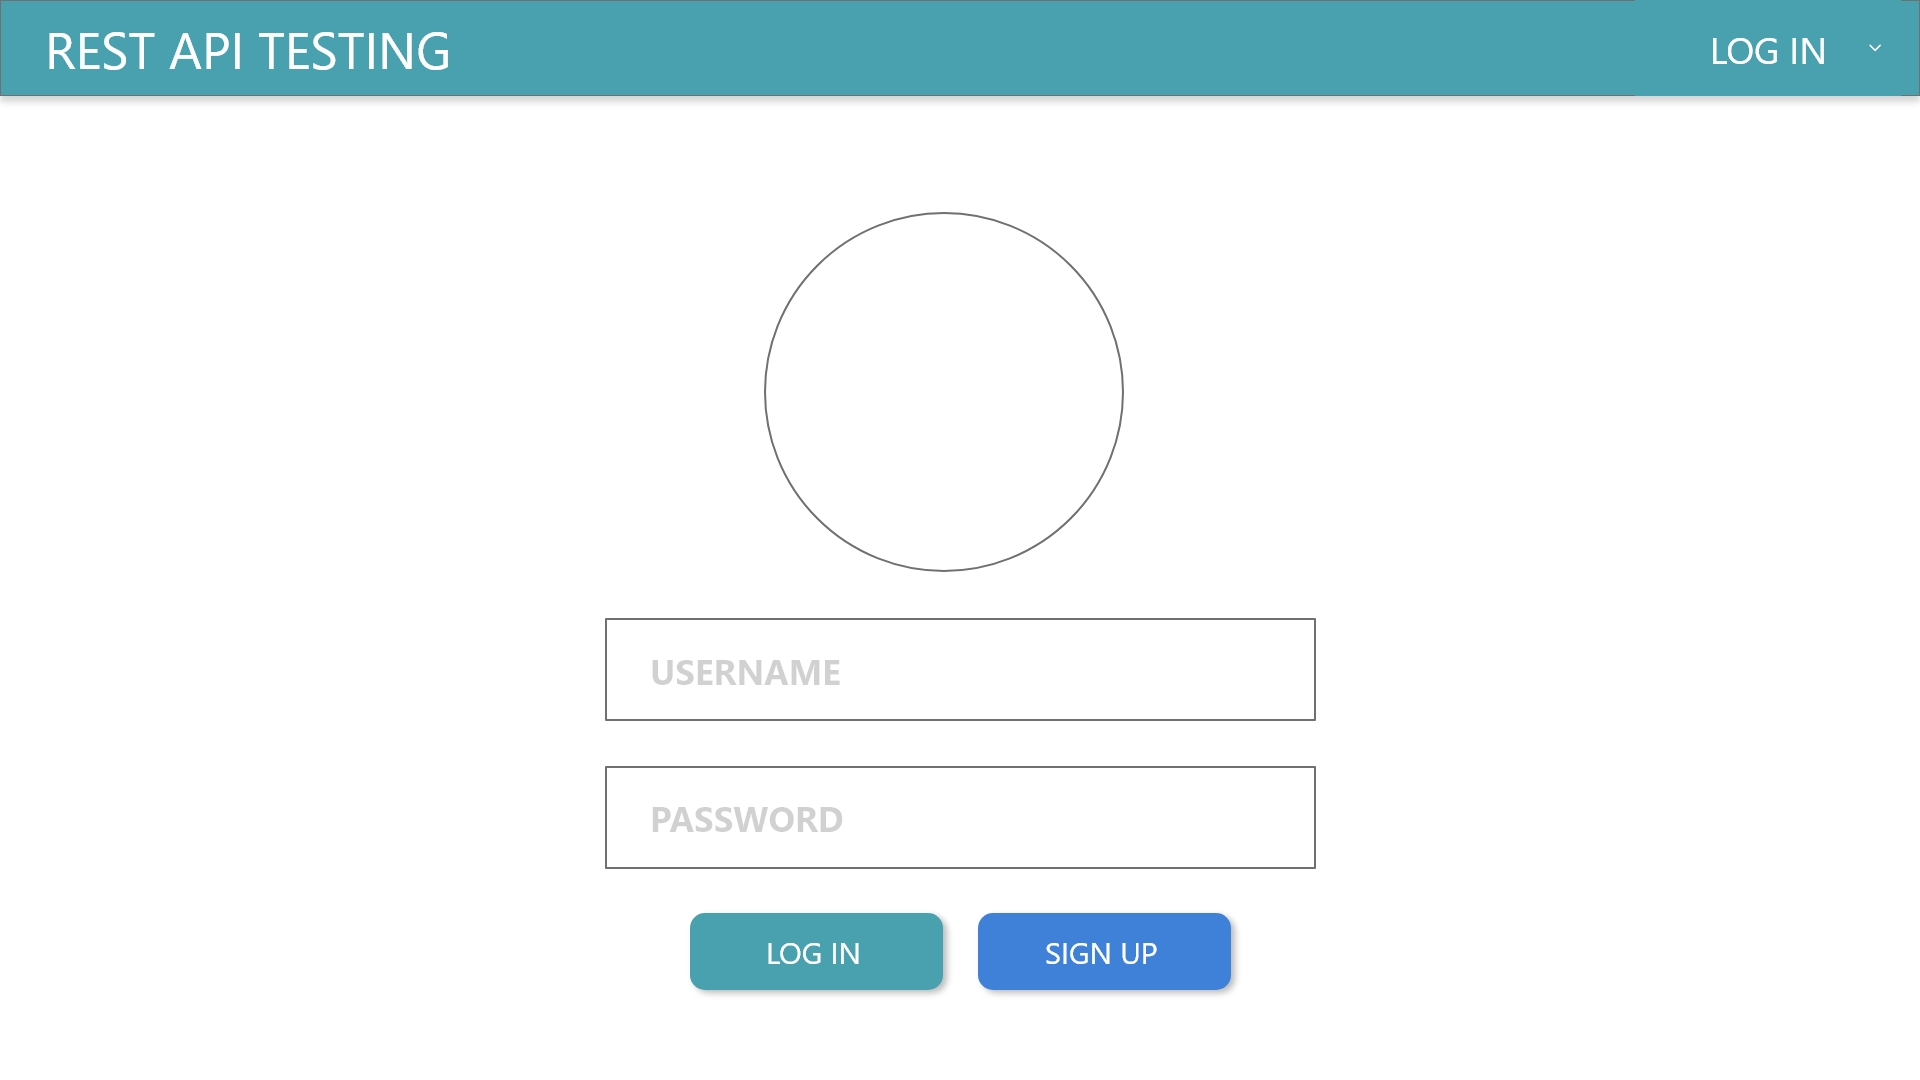
\includegraphics[width=5in]{latex/figures/loginxd.jpg}
	\caption{ตัวอย่างการออกแบบหน้า Log in}
	\label{fig:loginxd}
\end{figure}

\begin{figure}[!thb]
	\captionsetup{justification=centering}
	\centering
	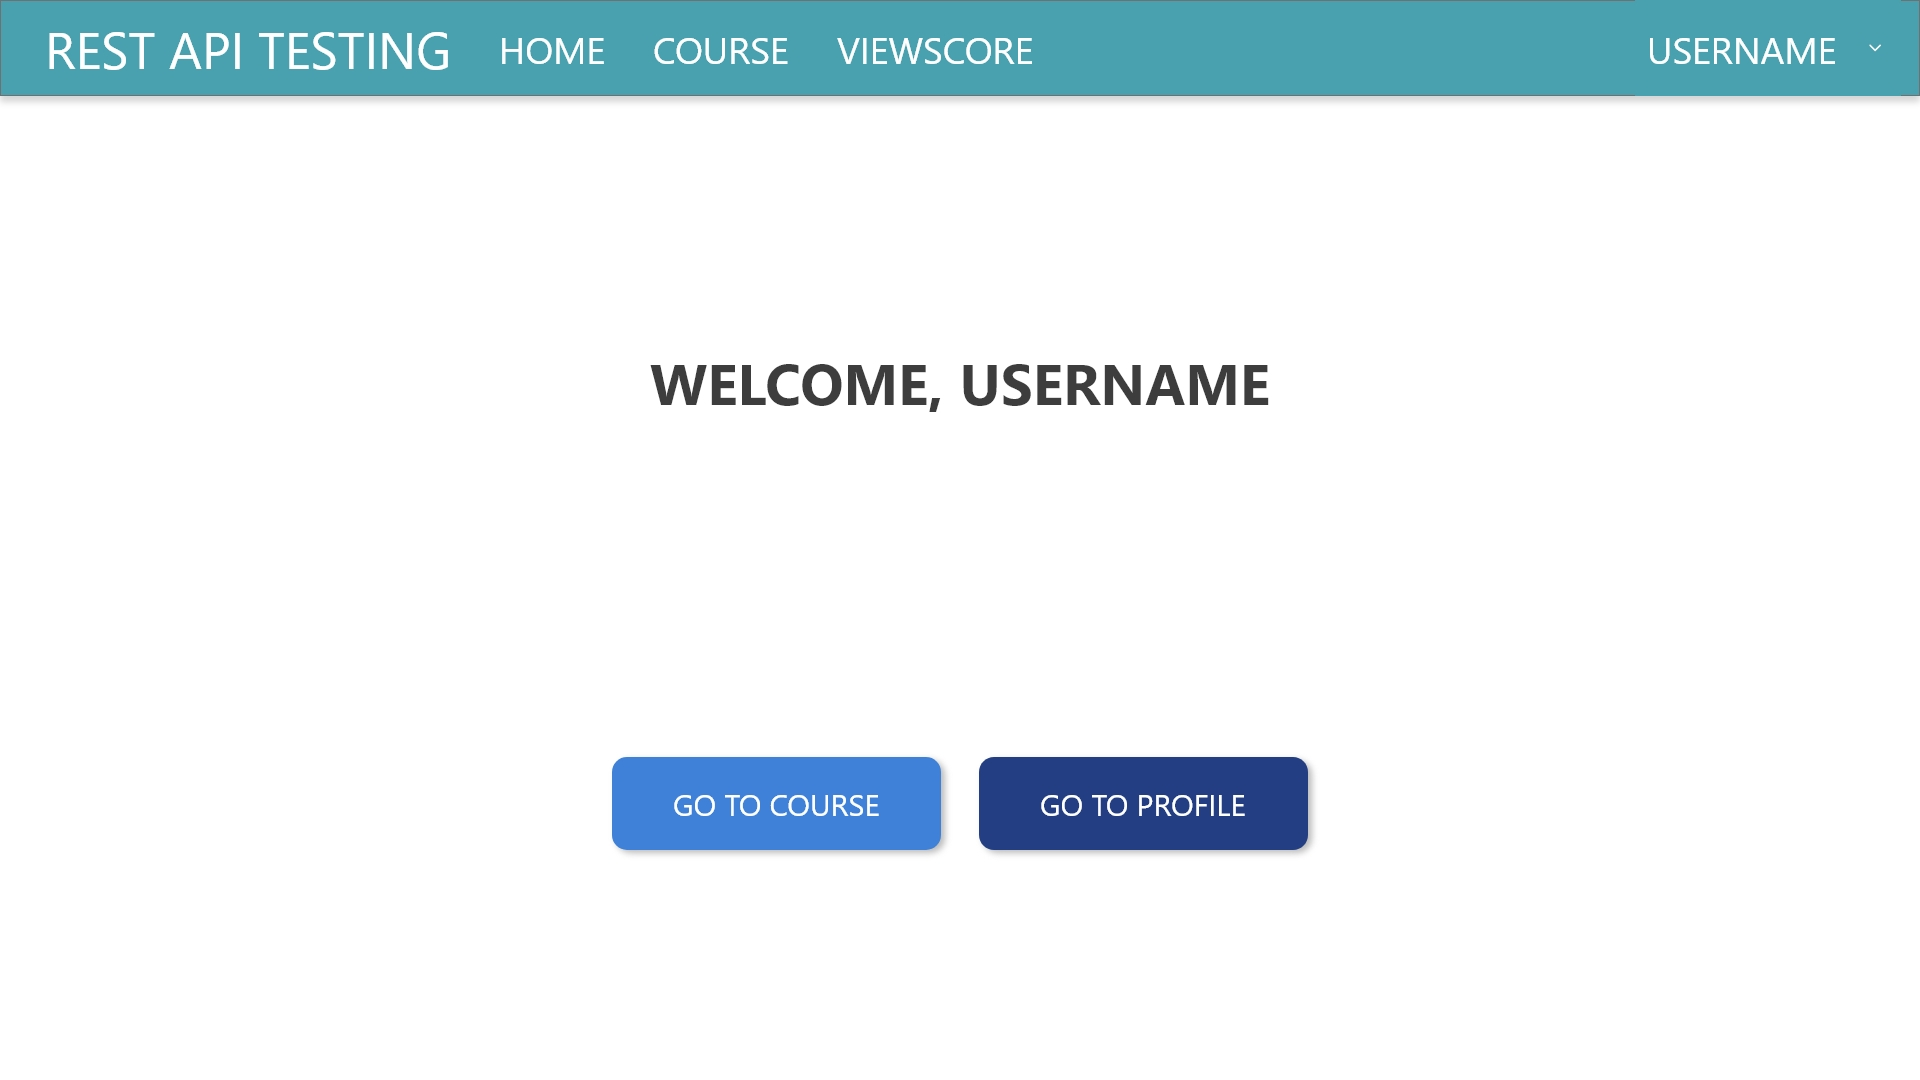
\includegraphics[width=5in]{latex/figures/homepagexd.jpg}
	\caption{ตัวอย่างการออกแบบหน้า Homepage}
	\label{fig:hompagexd}
\end{figure}
\newpage

\begin{figure}[!thb]
	\captionsetup{justification=centering}
	\centering
	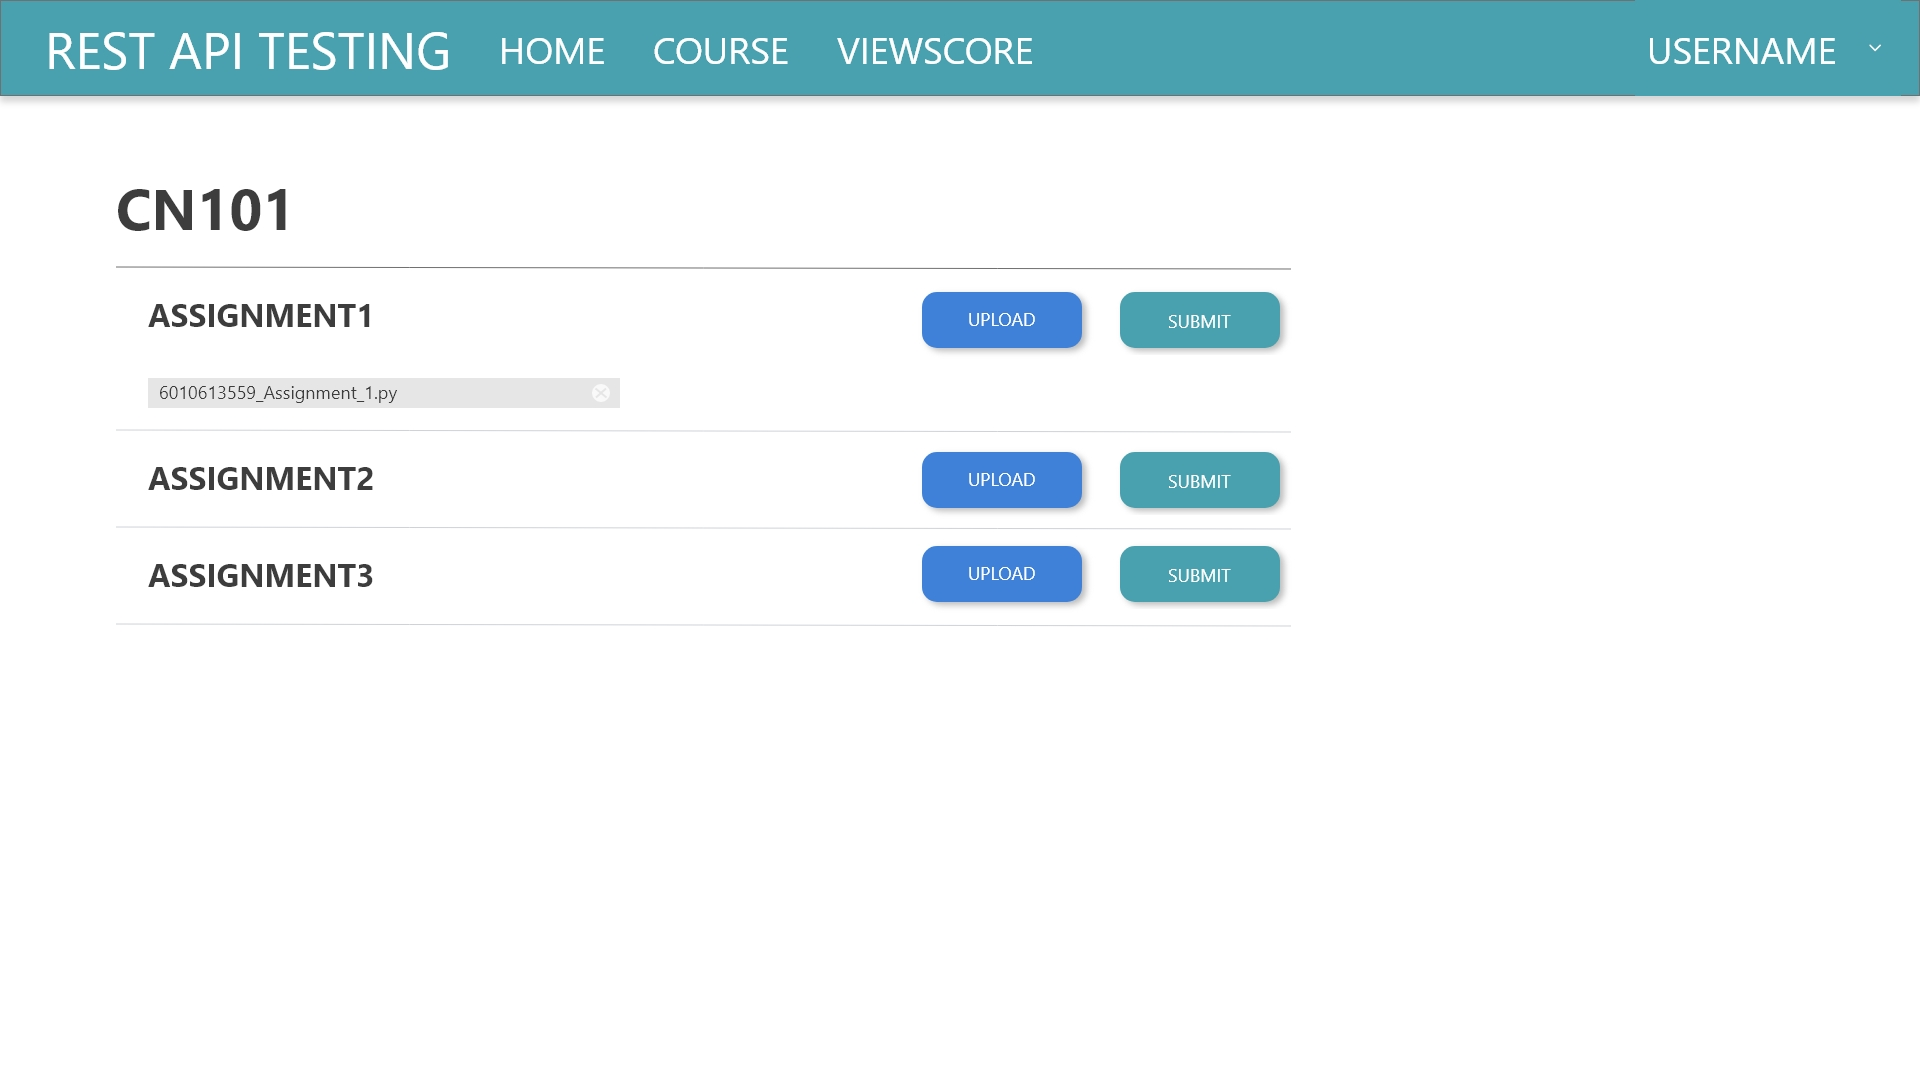
\includegraphics[width=5in]{latex/figures/assignmentxd.jpg}
	\caption{ตัวอย่างการออกแบบหน้า Assignment}
	\label{fig:assignmentxd}
\end{figure}

\begin{figure}[!thb]
	\captionsetup{justification=centering}
	\centering
	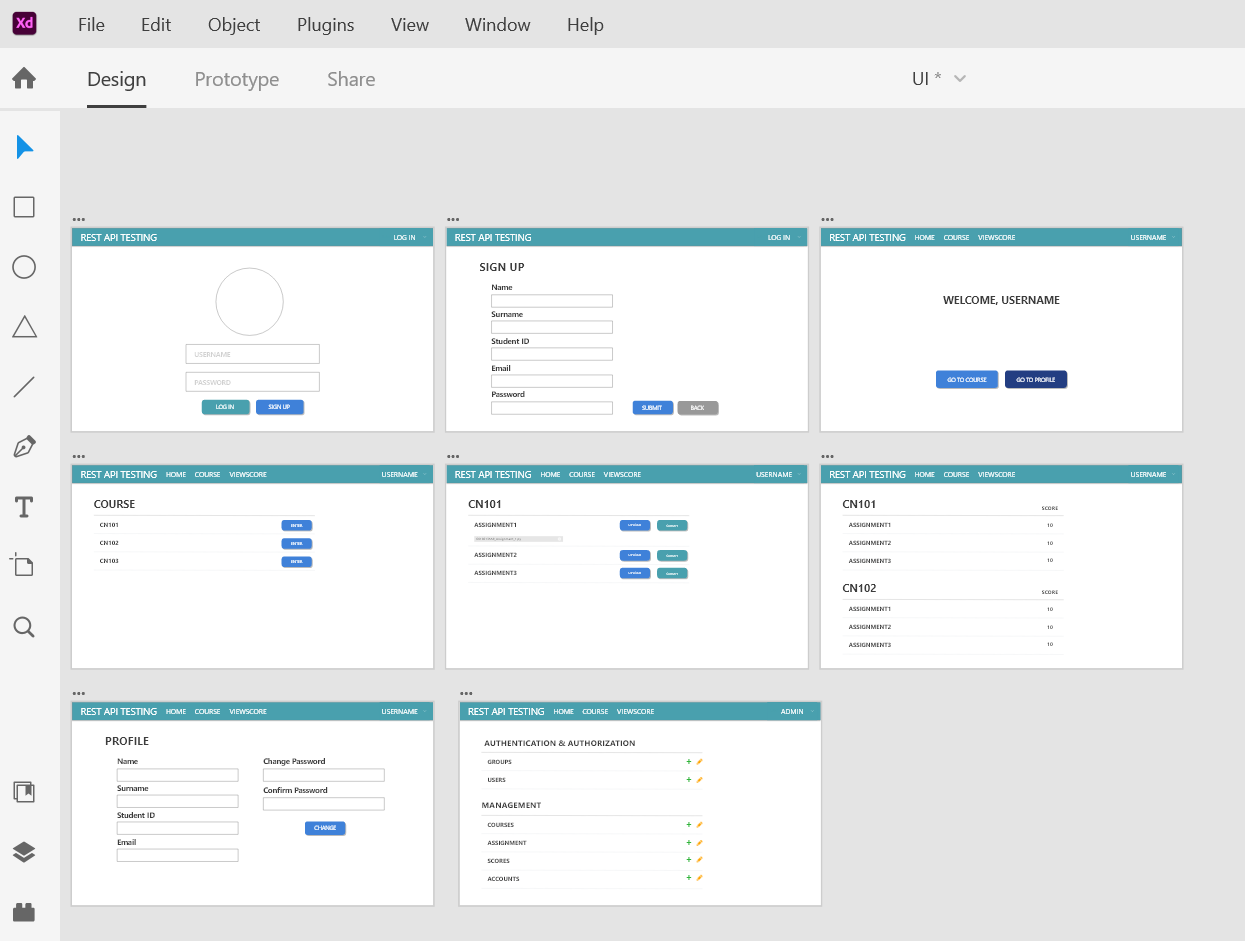
\includegraphics[width=5in]{latex/figures/mockup.png}
	\caption{ตัวอย่างการออกแบบหน้าต่าง ๆ โดยรวม}
	\label{fig:mockup}
\end{figure}
\newpage

\subsection{ภาษาคอมพิวเตอร์}
ภาษาที่เลือกใช้ในการเขียน Website คือภาษา HTML และ Python เนื่องจากภาษา Python มีการใช้งานอย่างแพร่หลาย จึงทำให้ง่ายต่อการเรียนรู้และศึกษา

\subsection{Django Framework}
ในการสร้าง Website ครั้งนี้ได้เลือกใช้ Django Framework เนื่องจาก
ทำงานได้รวดเร็ว มีเครื่องมือให้เลือกใช้ครบ

\subsubsection{การติดตั้ง Django}
หลังจากที่ทำการติดตั้ง Python เรียบร้อยแล้วก่อนจะทำการติดตั้ง Django ได้ทำการติดตั้ง Virtualenv เพื่อแยกสภาพแวดล้อมในการทำงานก่อน 
\begin{itemize}
    \item คำสั่ง pip install virtualenv
    \item และคำสั่ง virtualenv <ชื่อที่ต้องการ>
\end{itemize}
จากนั้นติดตั้ง django ด้วยคำสั่ง 
\begin{itemize}
    \item pip install django ใน virtualenv ที่เราได้ทำการสร้างขึ้น
\end{itemize}
ทำการสร้างโปรเจ็กต์ด้วยคำสั่งและเปิด server 
\begin{itemize}
    \item django-admin startproject <ชื่อโปรเจ็กต์>
    \item python manage.py runserver
\end{itemize}
ทดสอบด้วย http://localhost:8000 ก็จะสามารถเรียก server ขึ้นมาใช้งานได้

\subsubsection{การตั้งค่าการใช้งาน Admin Site}
เนื่องจาก Django Framework มีระบบ Django Administration มาให้สามารถใช้งานอยู่แล้ว จึงสะดวกในการใช้งานมากขึ้น
ในการเปิดใช้งาน Admin Site เริ่มจาก
\begin{itemize}
    \item การสร้าง superuser ด้วยคำสั่ง python manage.py createsuperuser
    \item จากนั้นระบบจะขึ้นให้ตั้งค่า Username และ password
\end{itemize}
เพียงเท่านี้ก็สามารถทำการ Log in ใช้งานหน้าของ Admin Site ได้
\newpage

\begin{figure}[!thb]
	\captionsetup{justification=centering}
	\centering
	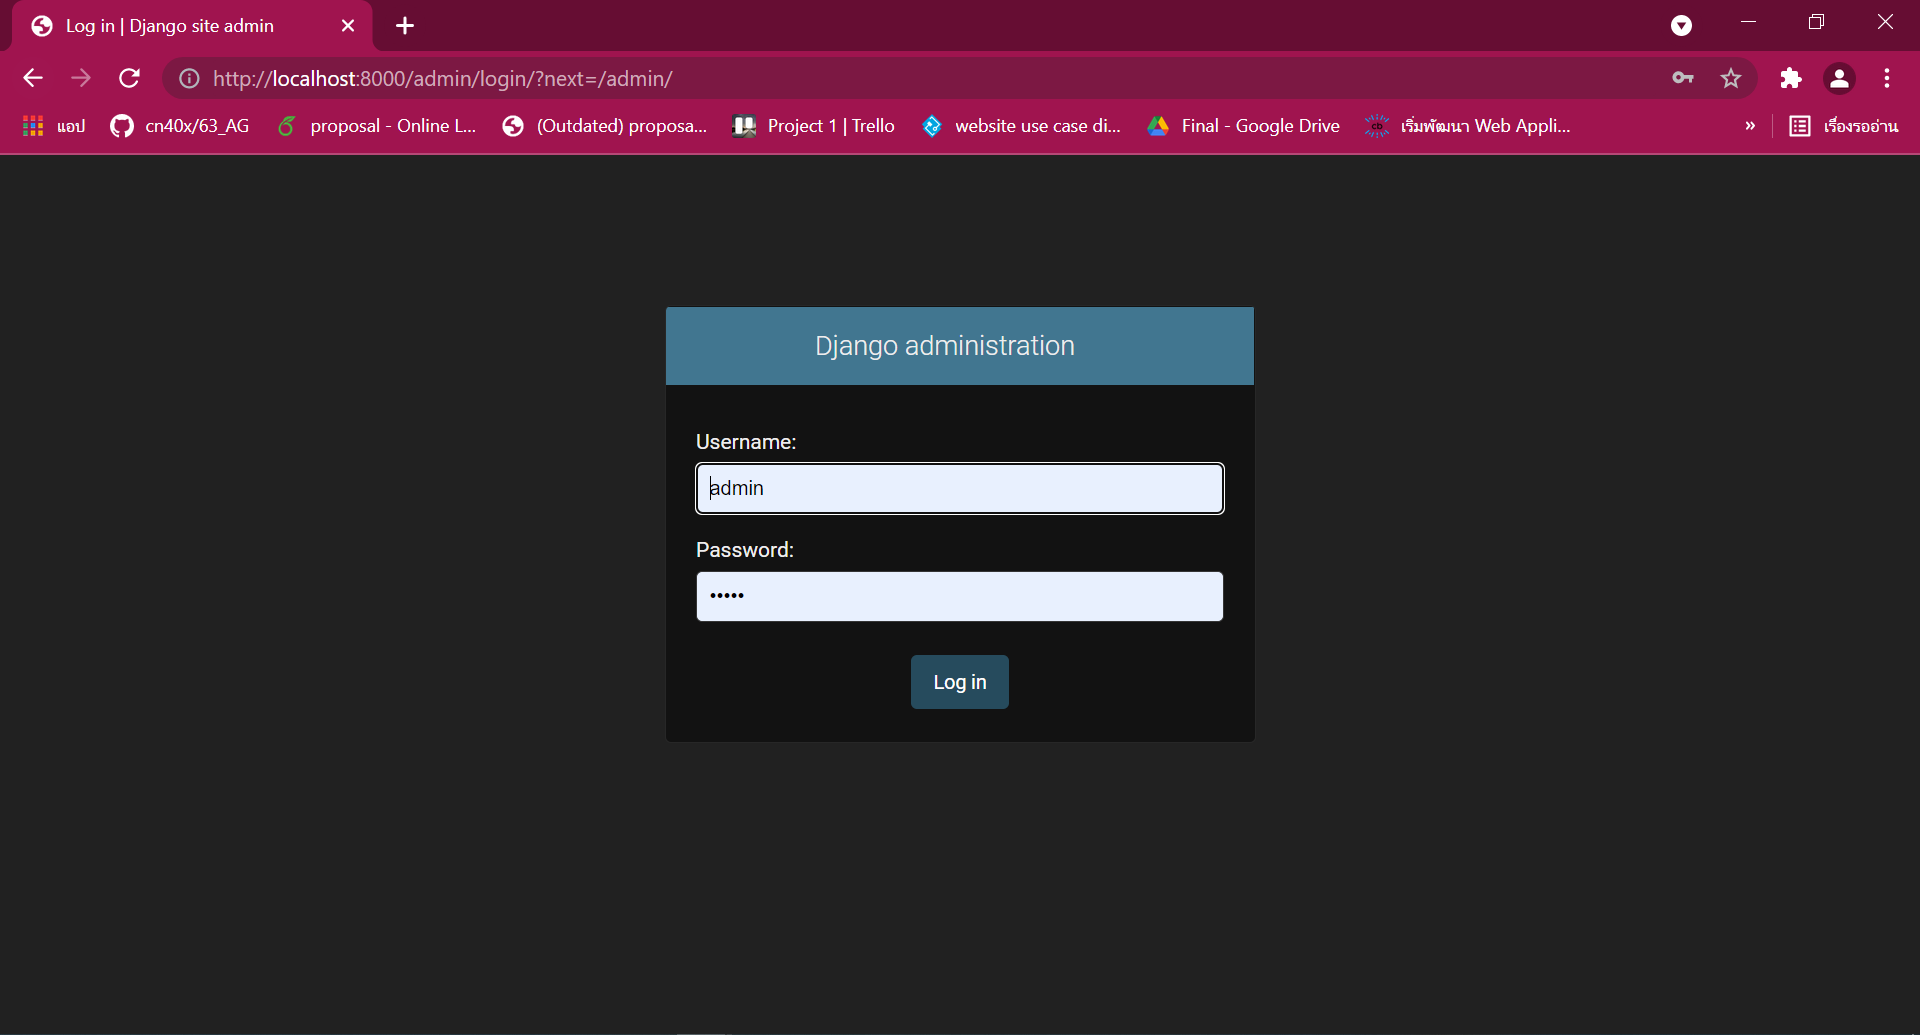
\includegraphics[width=5in]{latex/figures/admin.png}
	\caption{ภาพจากหน้าเว็บ Admin Site}
	\label{figure:admin}
\end{figure}

\begin{figure}[!thb]
	\captionsetup{justification=centering}
	\centering
	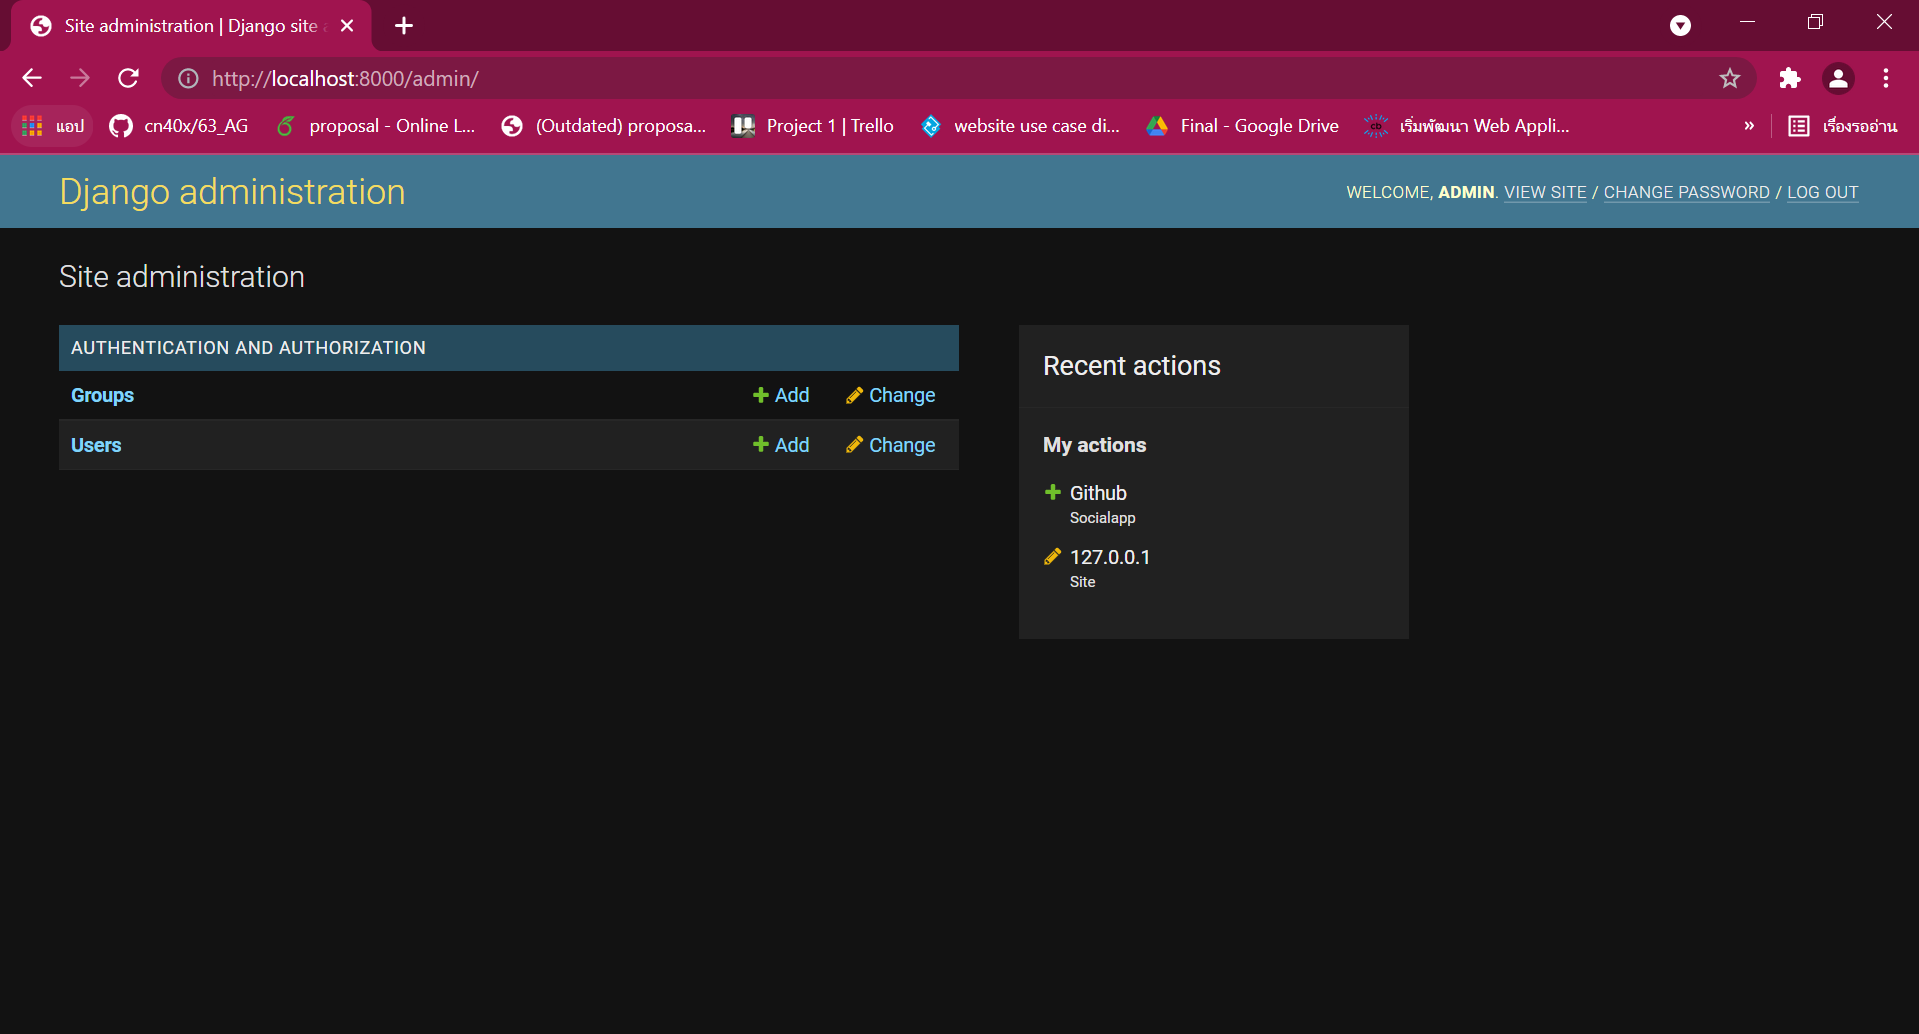
\includegraphics[width=5in]{latex/figures/adminlogin.png}
	\caption{ภาพหน้าเว็บเมื่อทำการ Log in เสร็จสิ้น}
	\label{figure:adminlogin}
\end{figure}
\newpage

\subsection{Website สำหรับใช้งานจริง}
เริ่มต้นการเขียนเว็บด้วยโปรแกรม Virtual Studio Code
โดยรูปแบบการทำงานของ Django จะเป็นแบบ Model View Template (MVT)
\begin{figure}[!thb]
	\captionsetup{justification=centering}
	\centering
	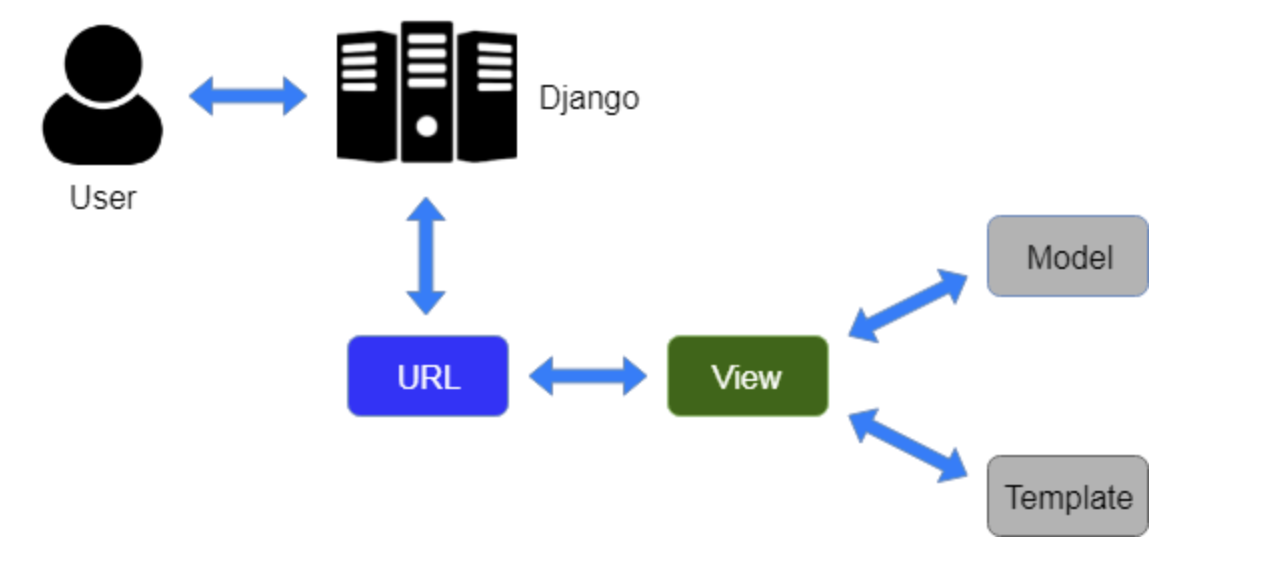
\includegraphics[width=5in]{latex/figures/mvt.png}
	\captionsource{Model-View-Template}{\url{https://www.javatpoint.com/django-mvt}}
	\label{figure:mvt}
\end{figure}

\begin{itemize}
    \item Model คือส่วนที่เก็บข้อมูลของ Application
    \item View สำหรับประมวลผลคำสั่งหรือข้อมูลต่างๆ (เหมือนกับ Controller) และส่งไปแสดงผลตรงส่วนของ Template
    \item Template คือหน้าตา Application ประมวลผลจาก View มาแสดงผลหน้าเว็บร่วมกับ HTML
\end{itemize}

\newpage
หลังจากที่ทำการ startproject ไปในขั้นตอนของการติดตั้งเรียบร้อยแล้ว โครงสร้างของโปรเจ็กต์จะเป็นรูปแบบดังนี้

\begin{figure}[!thb]
	\captionsetup{justification=centering}
	\centering
	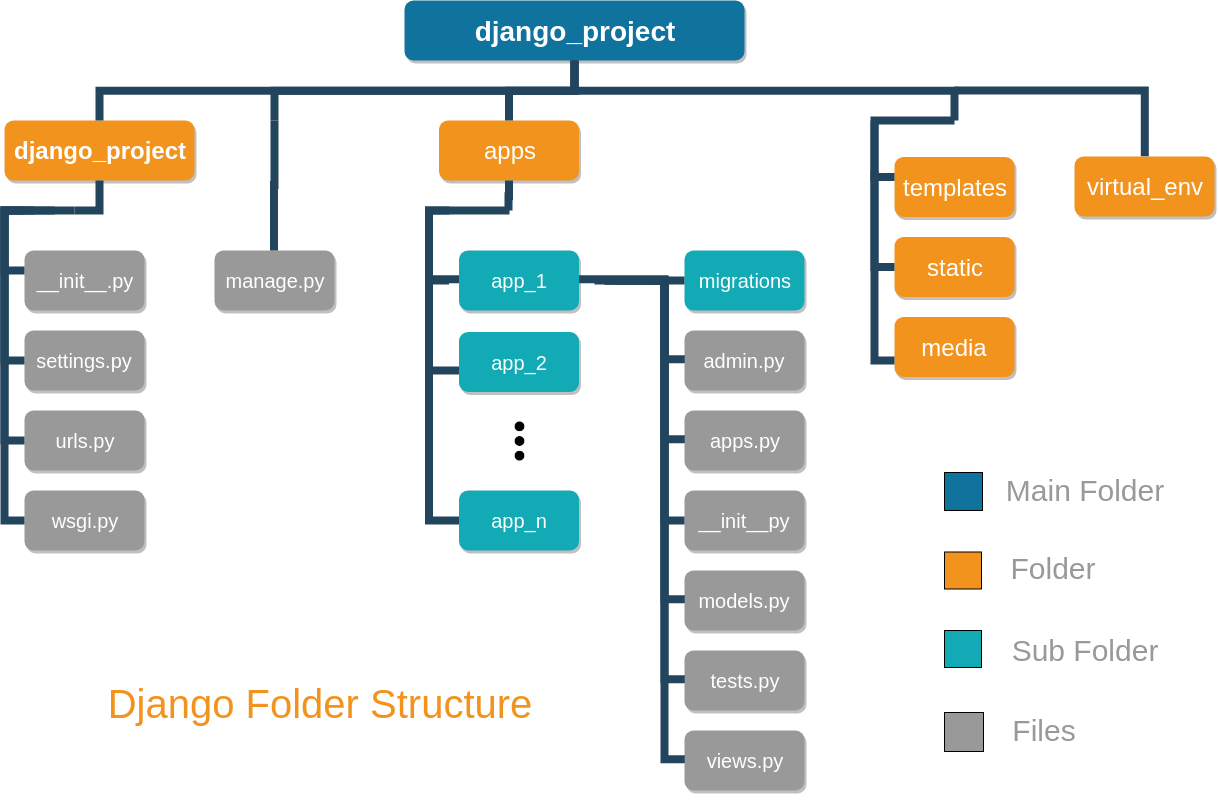
\includegraphics[width=6in]{latex/figures/djangoproject.png}
	\captionsource{Django Project Structure}{\url{https://studygyaan.com/django/best-practice-to-structure-django-project-directories-and-files}}
	\label{fig:djangoproject}
\end{figure}
\newpage

ในการดำเนินงานเบื้องต้นได้ทำการเขียนเว็บในส่วนของ template หน้าต่างๆ  สามารถเชื่อมต่อหากันในแต่ละหน้าได้ และ สามารถ Runserver ขึ้นมาเพื่อใช้งานได้ดังนี้

\begin{figure}[!thb]
	\captionsetup{justification=centering}
	\centering
	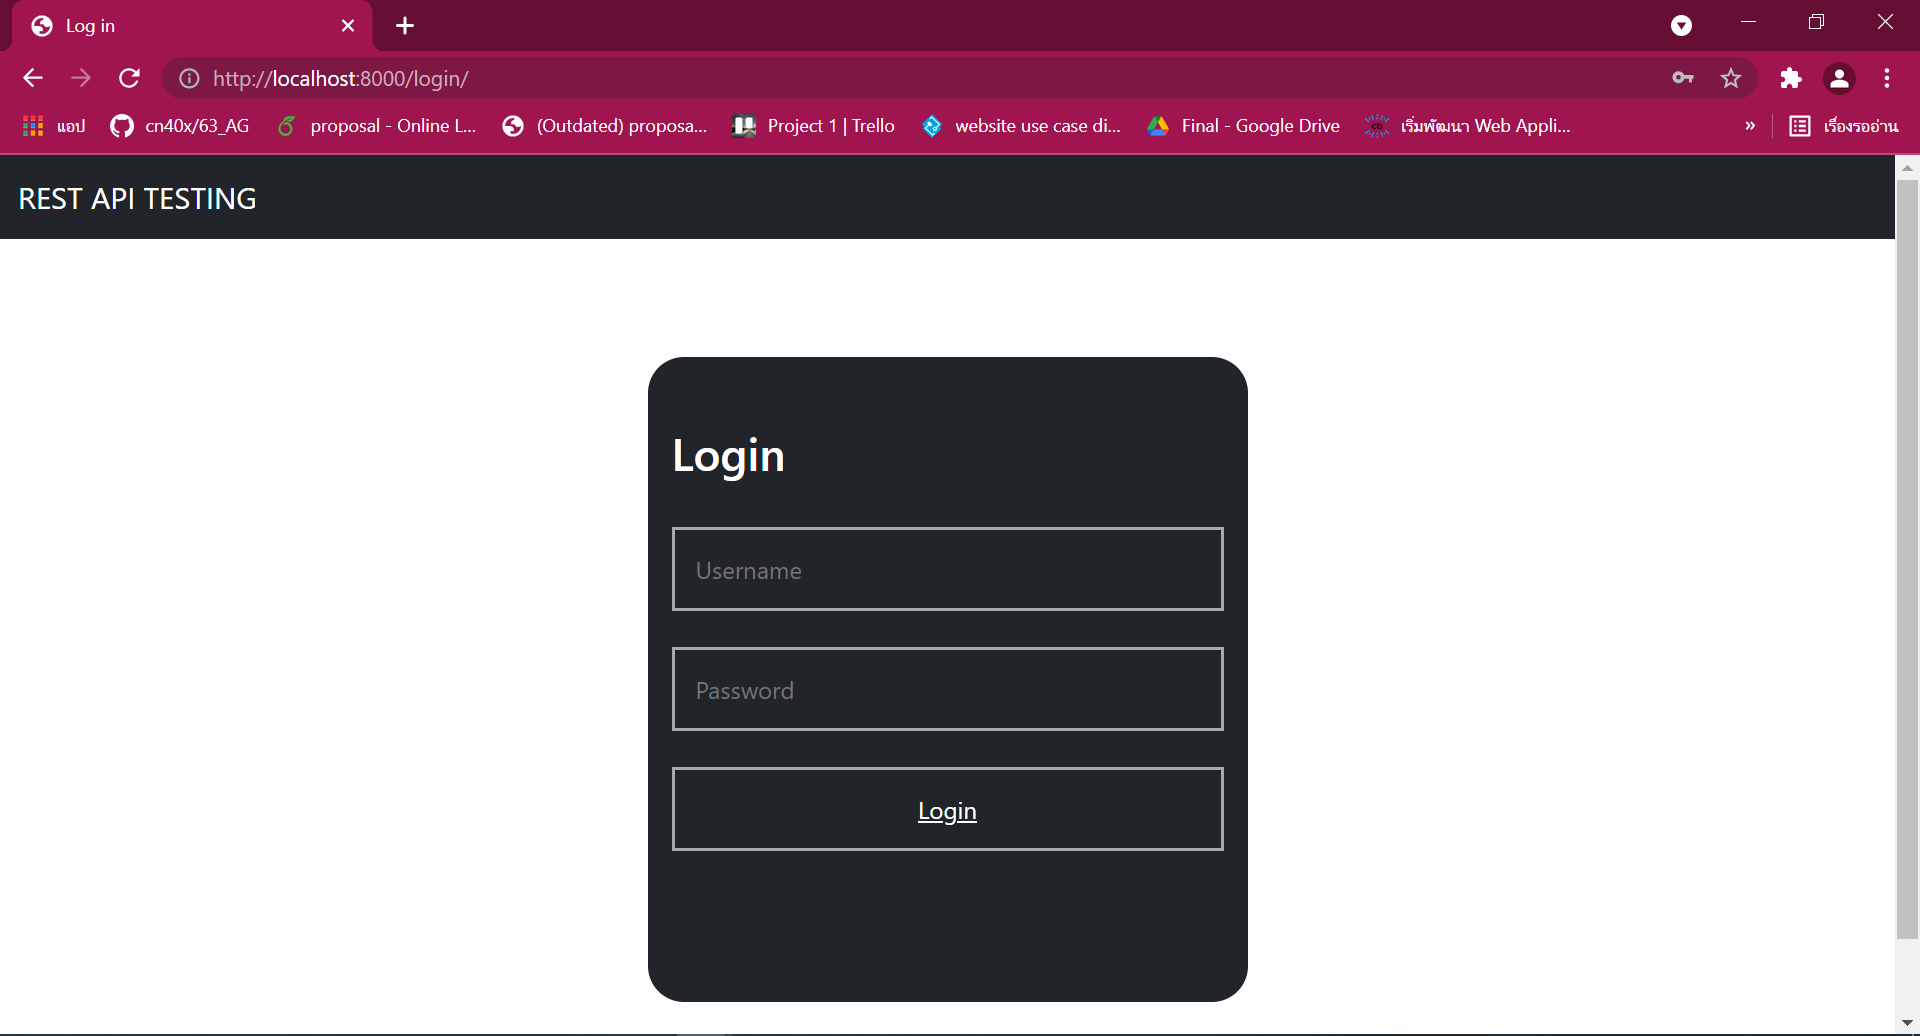
\includegraphics[width=5in]{latex/figures/login.png}
	\caption{รูปภาพในส่วนของหน้า Log in}
	\label{fig:login}
\end{figure}
\noindent จากรูปที่ \ref{fig:login} แสดงการเข้าถึงเว็บด้วยการ Log in ในส่วนนี้ยังไม่สามารถทำการ Log in ได้จริง ๆ เนื่องจากยังอยู่ในระหว่างการศึกษาเพื่อจะนำการ Authentication มาใช้ร่วม
\newline
\begin{figure}[!thb]
	\captionsetup{justification=centering}
	\centering
	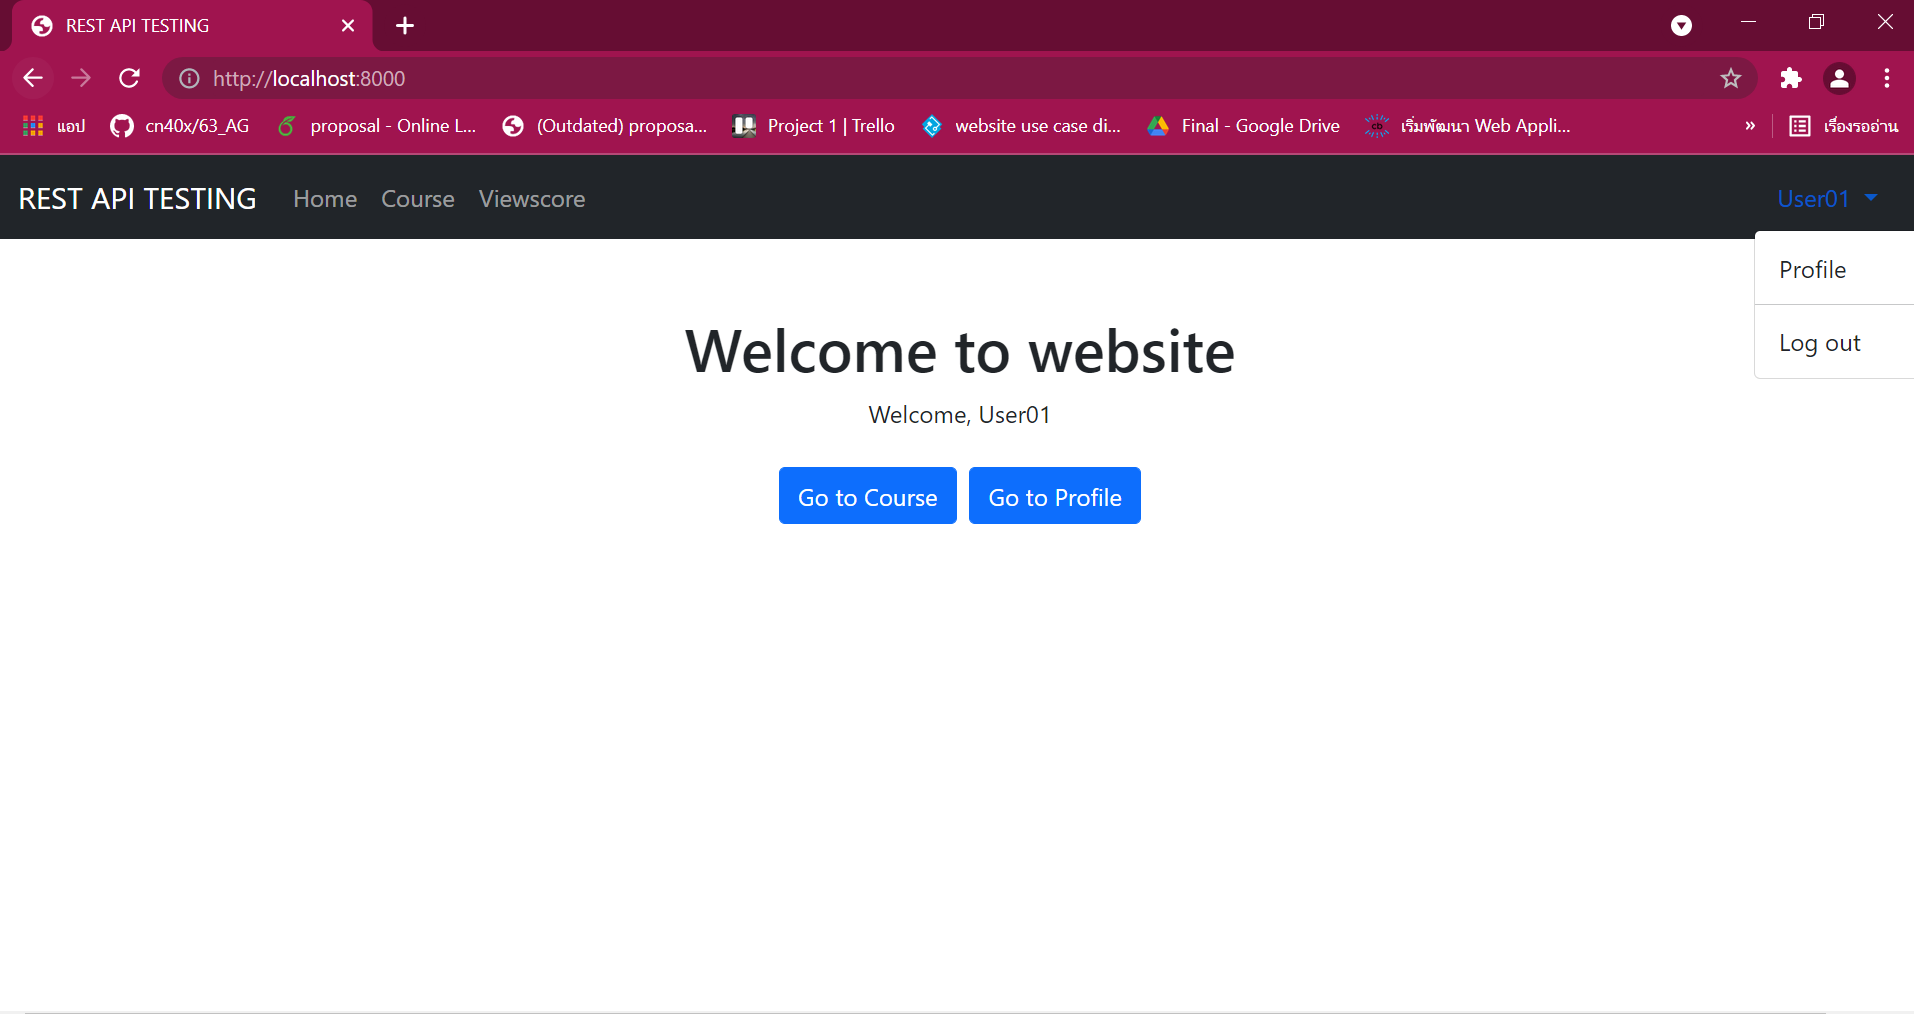
\includegraphics[width=5in]{latex/figures/home.png}
	\caption{รูปภาพในส่วนของหน้า Home}
	\label{fig:home}
\end{figure}
\newline
จากรูปที่ \ref{fig:home} เมื่อ Log in เข้ามาแล้วจะเจอกับหน้าหลักหรือหน้า Home ของเว็บ จากหน้านี้สามารถเข้าถึงหรือเชื่อมต่อไปยังหน้า template อื่น ๆ ได้
\newpage

\begin{figure}[!thb]
	\captionsetup{justification=centering}
	\centering
	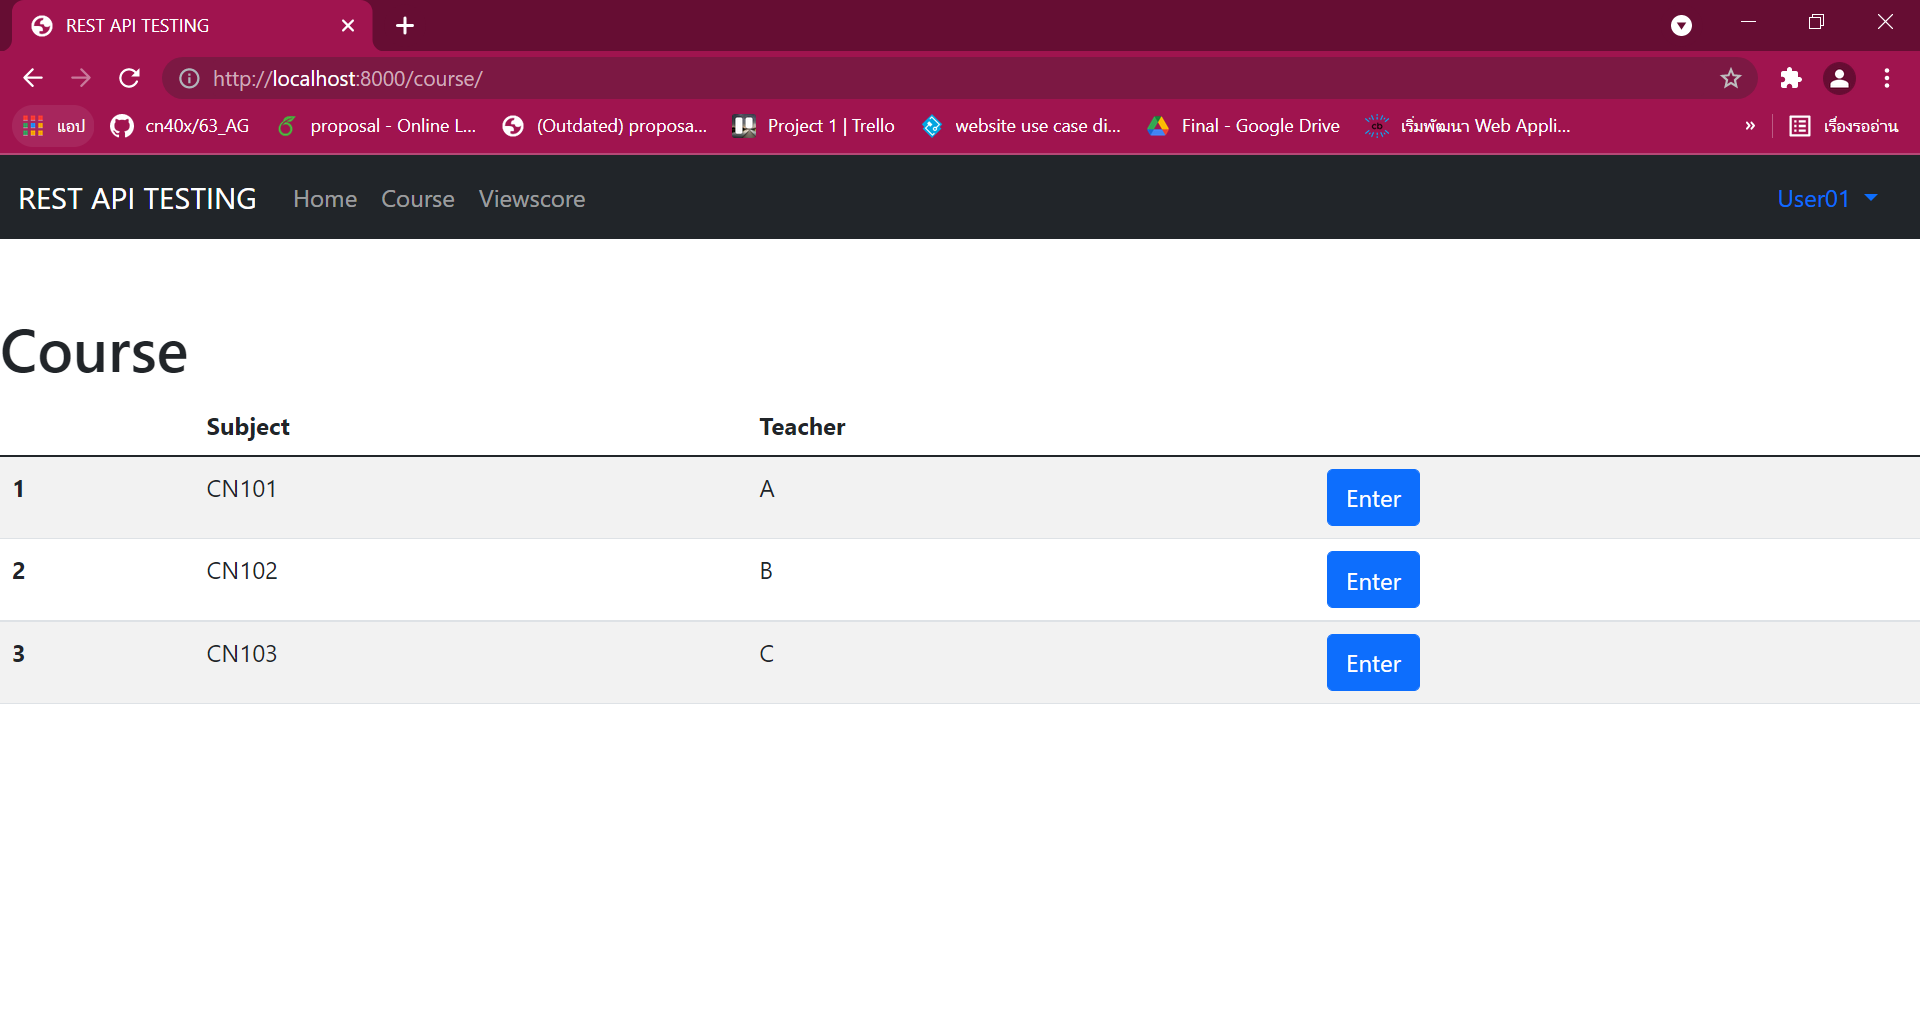
\includegraphics[width=5in]{latex/figures/course.png}
	\caption{รูปภาพในส่วนของหน้า Course}
	\label{fig:coure}
\end{figure}
\noindent จากรูปที่ \ref{fig:coure} ในหน้า Course หรือ
วิชาเรียนสามารถกดปุ่ม Enter เพื่อไปยังหน้า Assignment

\begin{figure}[!thb]
	\captionsetup{justification=centering}
	\centering
	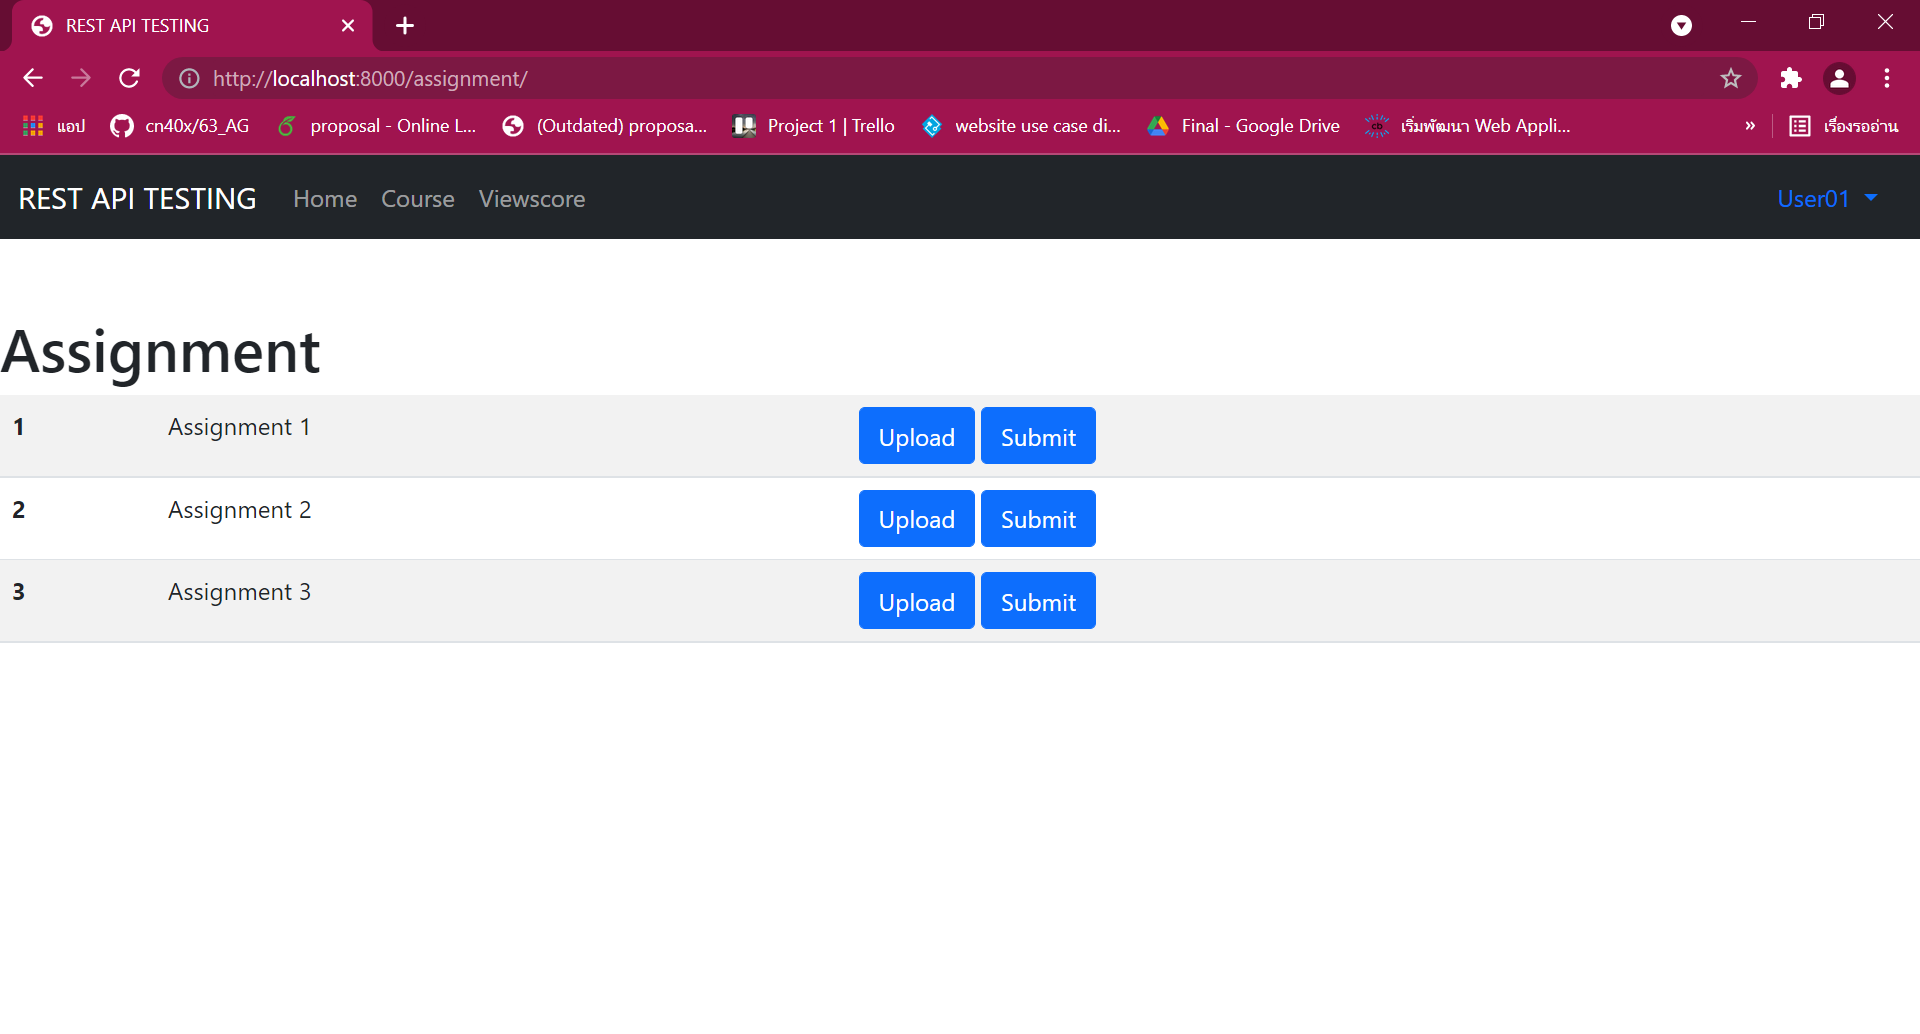
\includegraphics[width=5in]{latex/figures/assign.png}
	\caption{รูปภาพในส่วนของหน้า Assignment}
	\label{fig:assign}
\end{figure}
\noindent จากรูปที่ \ref{fig:assign} หน้า Assignment แสดงการบ้านต่าง ๆ สามารถกดปุ่ม upload เพื่อเลือกไฟล์จากเครื่องได้ ในส่วนนี้ยังไม่สามารถ upload ได้จริงเนื่องจากยังไม่มีฐานข้อมูลให้เก็บ และสามารถกดปุ่ม submit เพื่อไปยังหน้าของ Viewscore ได้
\newpage

\begin{figure}[!thb]
	\captionsetup{justification=centering}
	\centering
	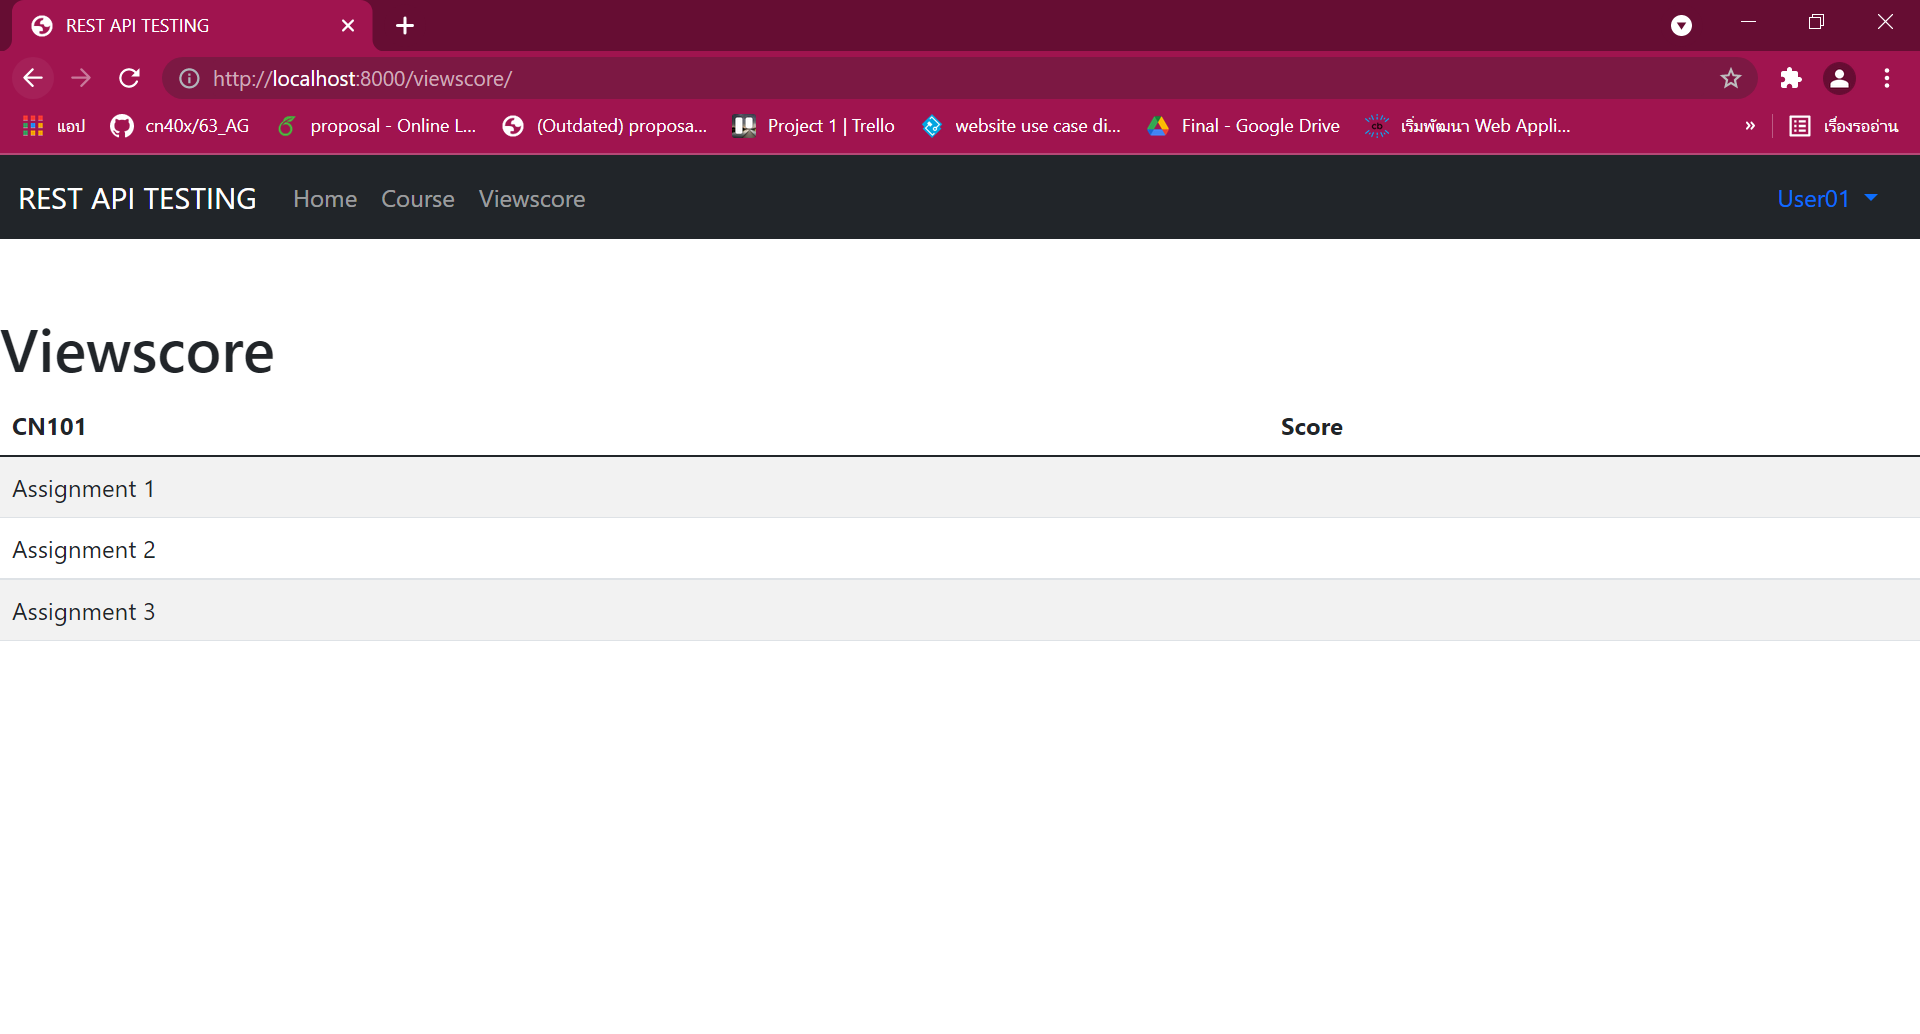
\includegraphics[width=5in]{latex/figures/score.png}
	\caption{รูปภาพในส่วนของหน้า View Score}
	\label{fig:score}
\end{figure}
\noindent จากรูปที่ \ref{fig:score} หน้า Viewscore จะเป็นหน้าที่ใช้ในการแสดงผลคะแนนของแต่ละ\mbox{การบ้าน}
\begin{figure}[!thb]
	\captionsetup{justification=centering}
	\centering
	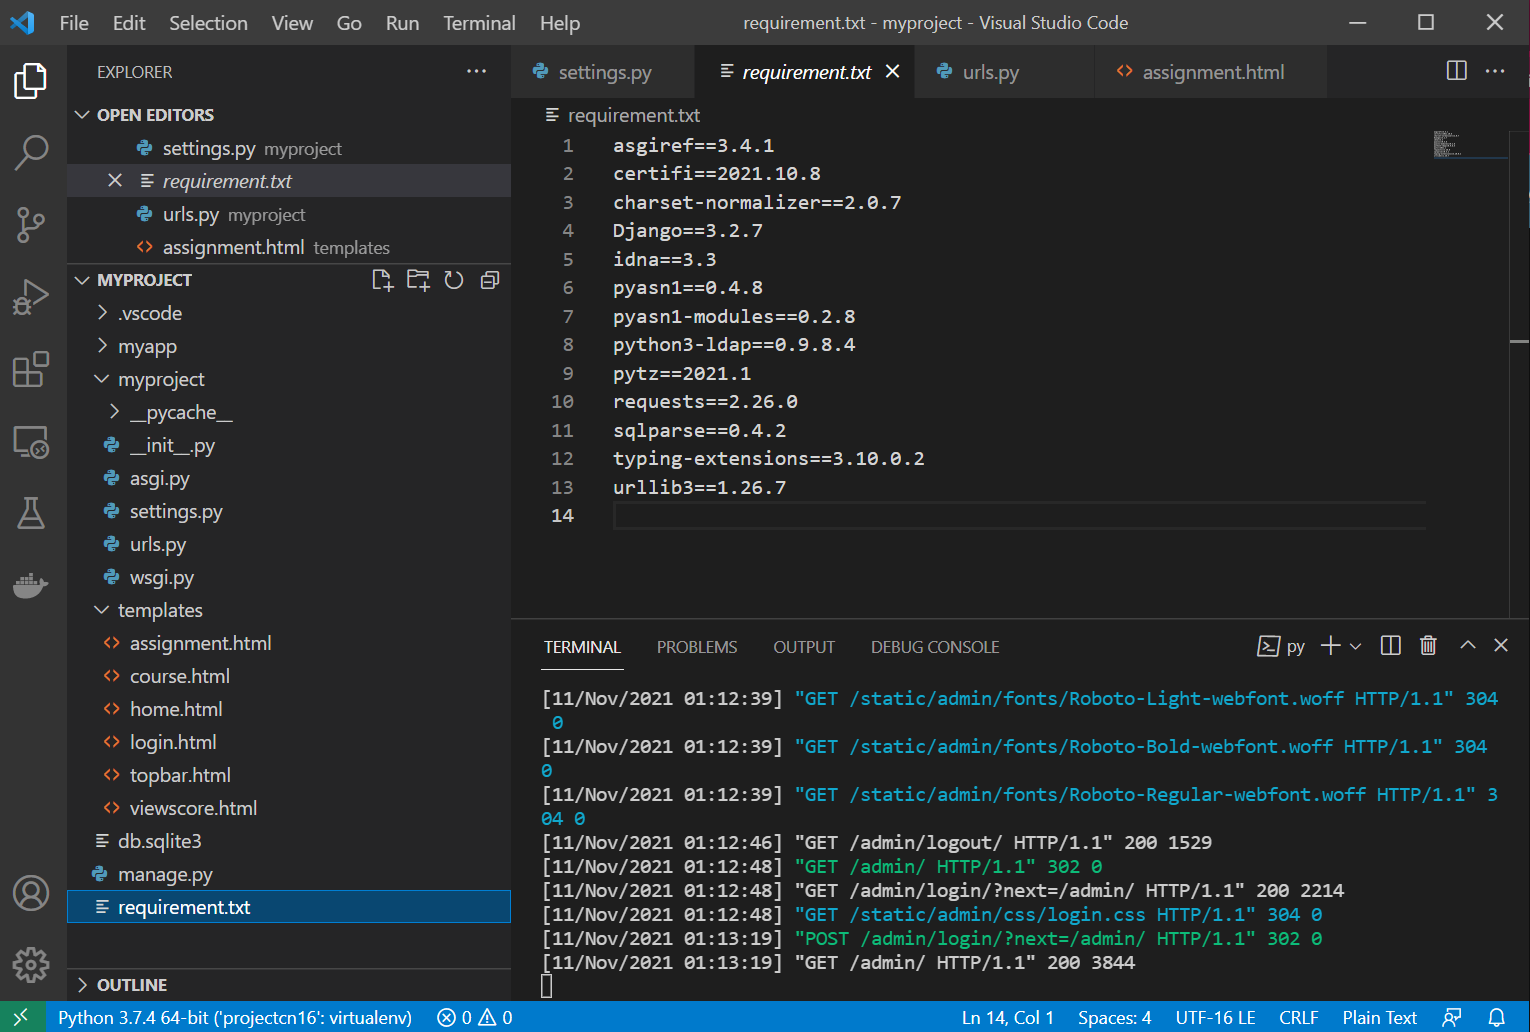
\includegraphics[width=5in]{latex/figures/code.png}
	\caption{แสดงโปรแกรมใน requirement.txt}
	\label{fig:code}
\end{figure}
\newline
จากรูปที่ \ref{fig:code} แสดงการติดตั้งโปรแกรมทั้งหมด ณ ปัจจุบันอยู่ในไฟล์ requirement.txt
\newpage

\section{ศึกษาการทำ Authentication ในการ Login }
โดยทั่วไปการใช้เว็บไซต์ แพลทฟอร์ม หรือ social media ต่าง ๆ ในโลกอินเตอร์เน็ต\mbox{จำเป็น}จะต้องมีการ Login เพื่อเข้าใช้งานและจะต้องมีการระบุตัวตนว่าผู้ใช้งานคนนี้เป็นใคร ด้วยการ Authentication

\subsection{Authentication คืออะไร}
Authentication คือ ระบบการยืนยันตัวตนที่เมื่อเราจะเข้าใช้งานในเว็บไซต์ \mbox{แอปพลิเคชัน}หรืออะไรก็ตามบนโลกออนไลน์เพื่อใช้ในการ Login
เราจะต้องสามารถยืนยันตัวตนได้โดยปกติจะใช้การยืนยันตัวตนจาก username และ password
\begin{figure}[!thb]
	\captionsetup{justification=centering}
	\centering
	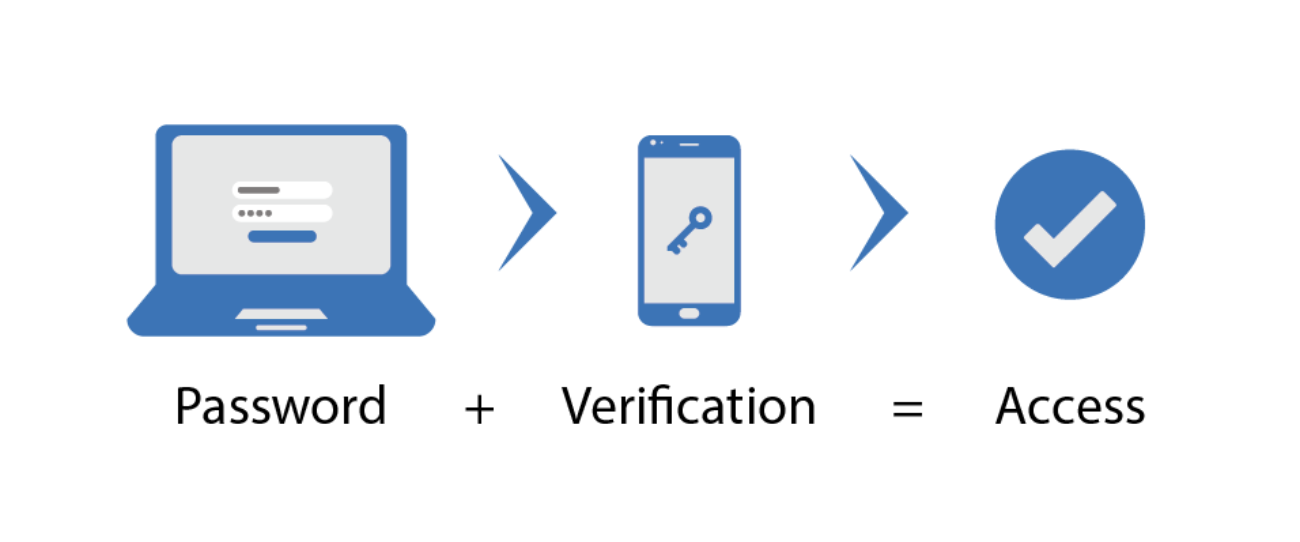
\includegraphics[width=6in]{latex/figures/authen.png}
	\captionsource{Authentication}{\url{https://medium.com/ingrammicroth/}}
	\label{fig:authen}
\end{figure}
\newpage

\subsection{Authentication โดยใช้ LDAP }
หน่วยงานจะจัดเก็บชื่อผู้ใช้ รหัสผ่าน ที่อยู่อีเมล และข้อมูลคงที่อื่นๆ ภายใน directory LDAP เป็นโปรโตคอลแอปพลิเคชันแบบเปิดและเป็นกลางสำหรับการเข้าถึงและบำรุงรักษาข้อมูลนั้น LDAP ยังสามารถจัดการกับการตรวจสอบสิทธิ์ ดังนั้นผู้ใช้สามารถลงชื่อเข้าใช้เพียงครั้งเดียวและเข้าถึงไฟล์ต่างๆ มากมายบนเซิร์ฟเวอร์ เนื่องจาก LDAP เป็นโปรโตคอล จึงไม่ระบุวิธีการทำงานของโปรแกรม directory แต่เป็นรูปแบบของภาษาที่ช่วยให้ผู้ใช้สามารถค้นหาข้อมูลที่ต้องการได้อย่างรวดเร็ว
\begin{flushleft}
	\textbf{ข้อดีของ LDAP}
\end{flushleft}
\begin{itemize}
    \item LDAP เก็บข้อมูลเป็นโครงสร้างแบบต้นไม้ ซึ่งสามารถเก็บข้อมูลแยกกันอยู่หลาย ๆ เครื่องได้โดยแยกตามโครงสร้างของต้นไม้
    \item LDAP สามารถทำงานได้ทั้งบนโปรโตคอลแบบ Secure และไม่ Secure
    \item ระบบ Authentication บน Linux สามารถใช้งานผ่าน LDAP ได้อย่างสมบูรณ์
    \item สามารถทำ Replication ได้
\end{itemize}


\begin{figure}[!thb]
	\captionsetup{justification=centering}
	\centering
	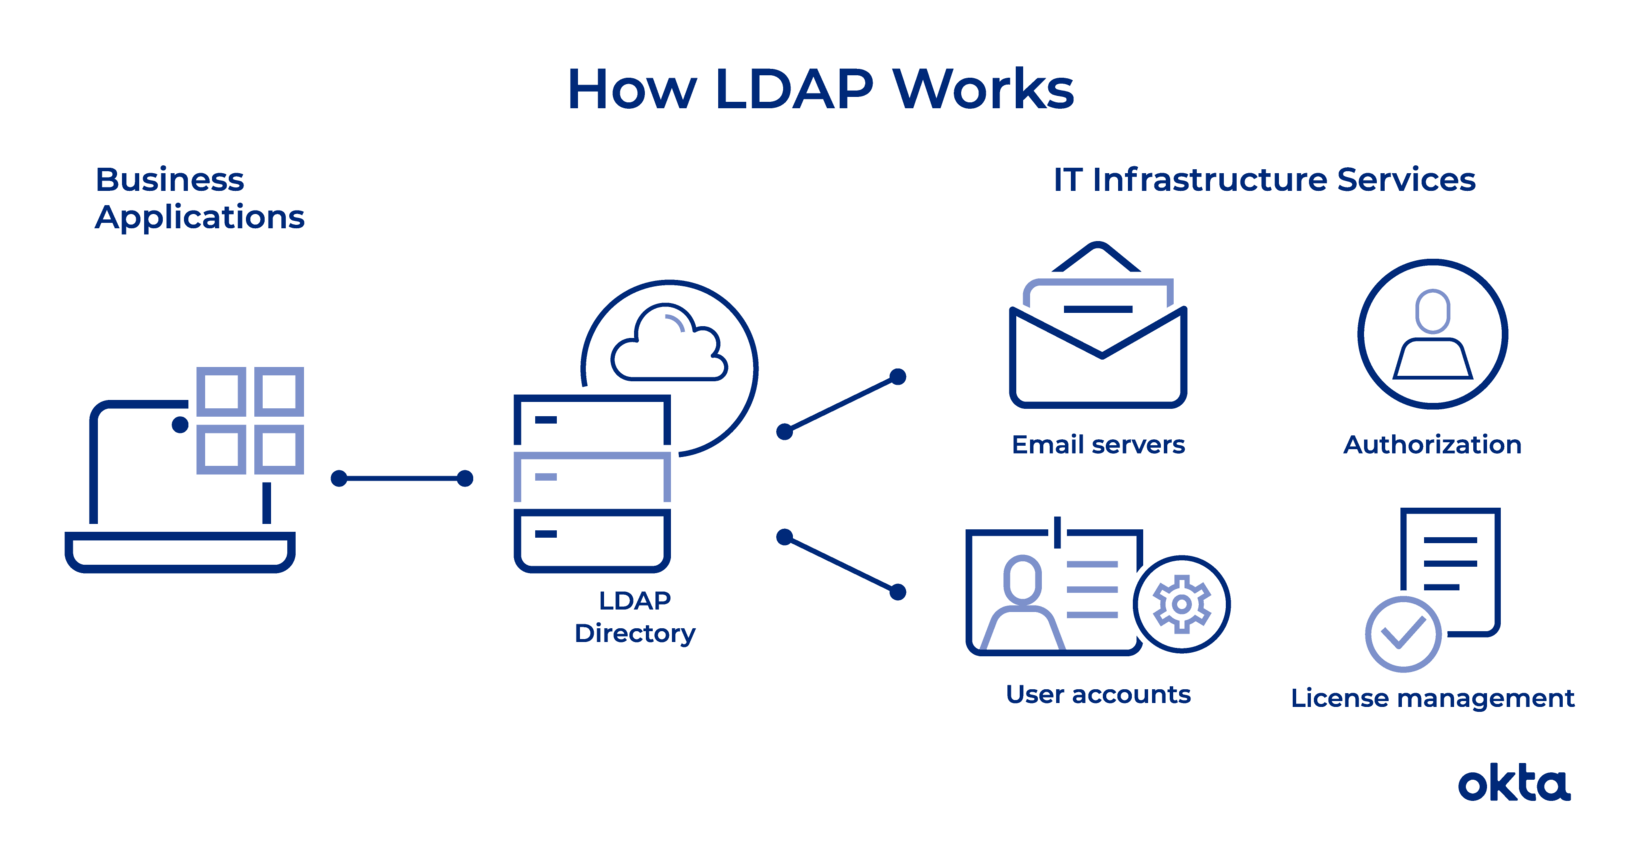
\includegraphics[width=6in]{latex/figures/ldap.png}
	\captionsource{LDAP Authentication}{\url{https://www.okta.com/identity-101/what-is-ldap/}}
	\label{fig:ldap}
\end{figure}
\newpage

\subsubsection{โครงสร้างของ LDAP Directory}
ตัว entry (ตำแหน่งข้อมูล) จะประกอบด้วยชุดของ attributes ทุก attribute จะมีชื่อ (type, description) ซึ่งจะกำหนดใน schema ทุก entry ต้องไม่ซ้ำกัน ซึ่งเป็น Distinguished Name (DN) cn คือ Common Name และ dc คือ Domain Component Server จะเก็บข้อมูลในลักษณะ subtree โดยจะเริ่มหาทีละ entry เช่น “dc=example,dc=com” โดย server อาจจะใช้ server อื่นเป็นตัวอ้างอิง เช่น “ou=department,dc=example,dc=com” อาจจะตอบกลับมาเป็น reference ไปที่ server ที่มีข้อมูลอยู่ในส่วนของ directory tree ซึ่งทาง client สามารถที่จะติดต่อกับ server อื่นได้
\begin{figure}[!thb]
    \captionsetup{justification=centering}
    \centering
    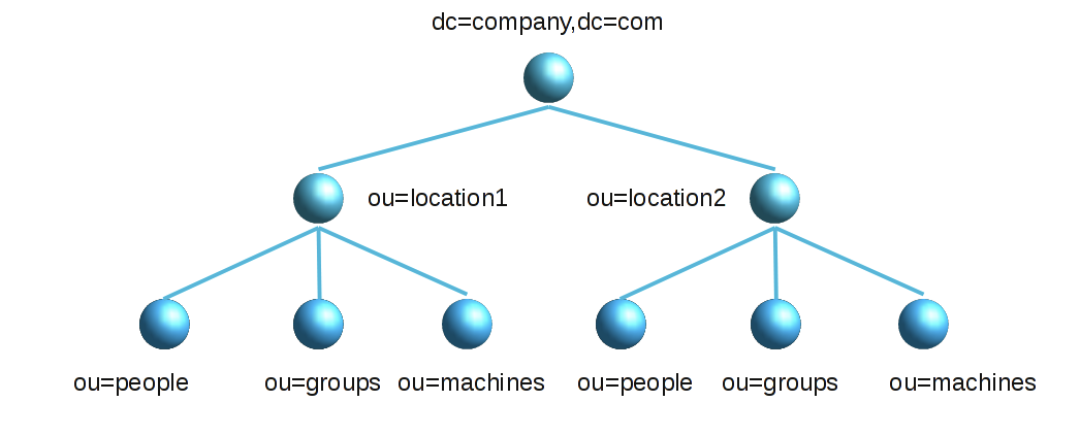
\includegraphics[width=5in]{latex/figures/ldap-structure.png}
    \captionsource{LDAP Structure}{\url{https://saixiii.com/what-is-ldap/}}
    \label{fig:ldap-structure}
\end{figure}
\newpage

\subsubsection{ตัวอย่างองค์ประกอบการ Coding ของ LDAP}
\begin{figure}[!thb]
\captionsetup{justification=centering}
\centering
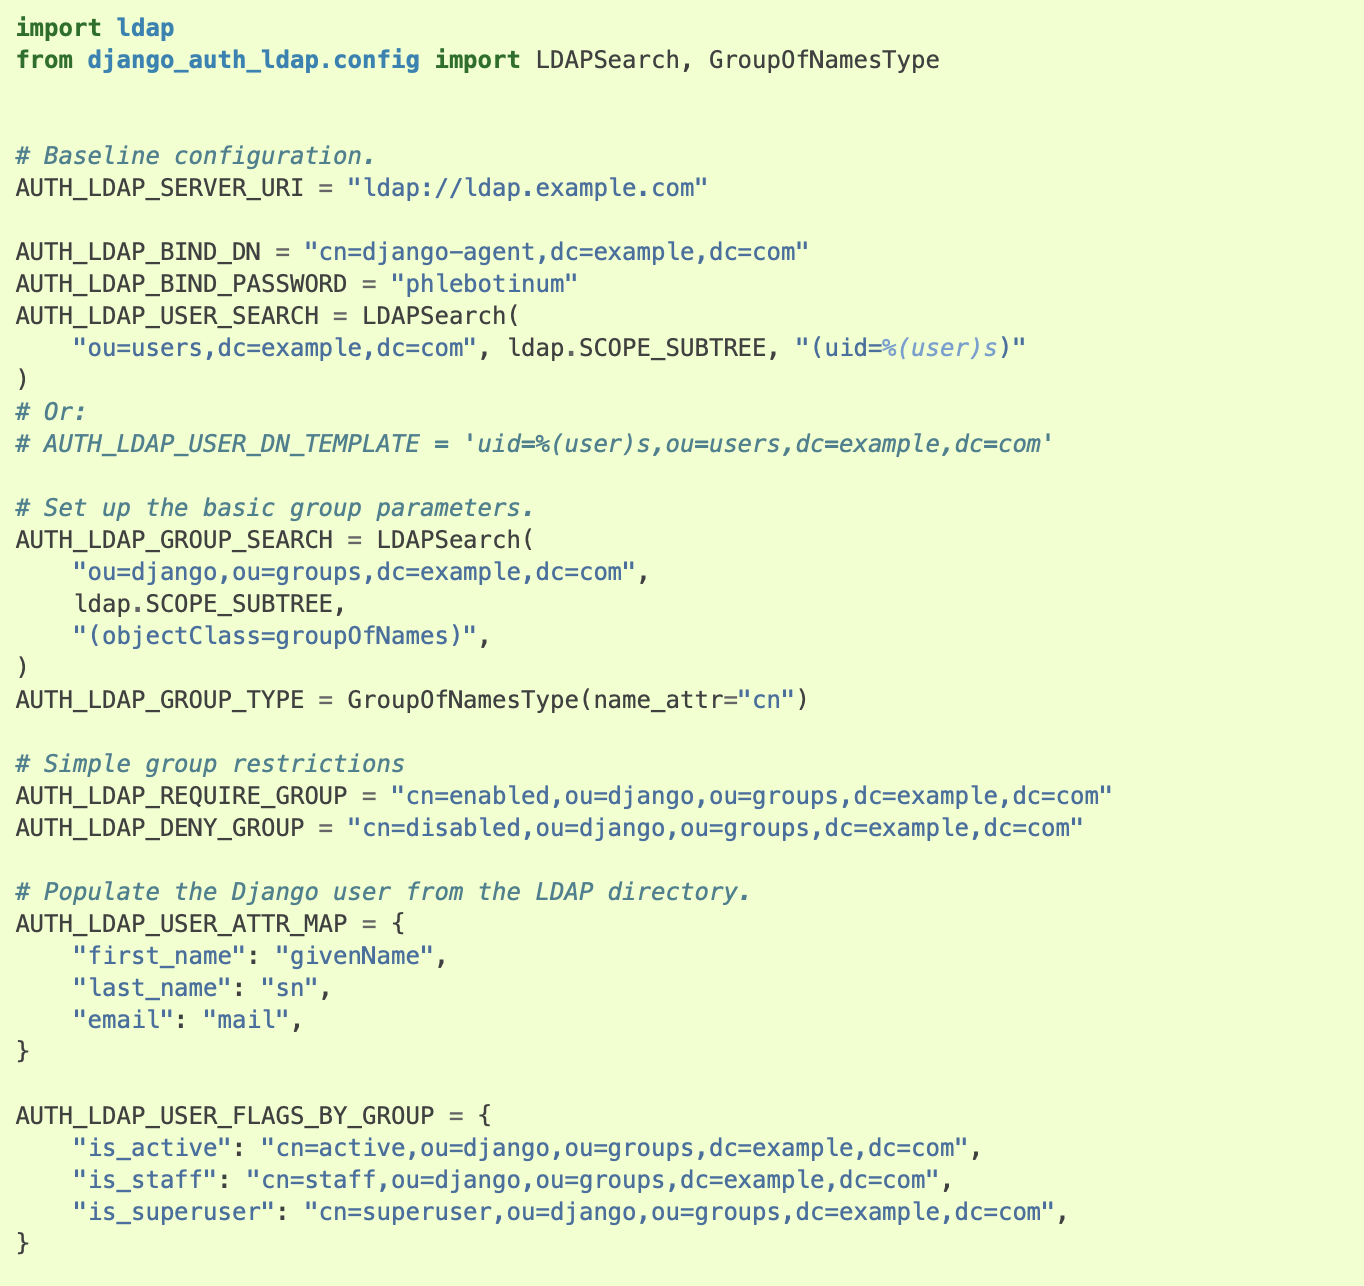
\includegraphics[width=6in]{figures/exam1}
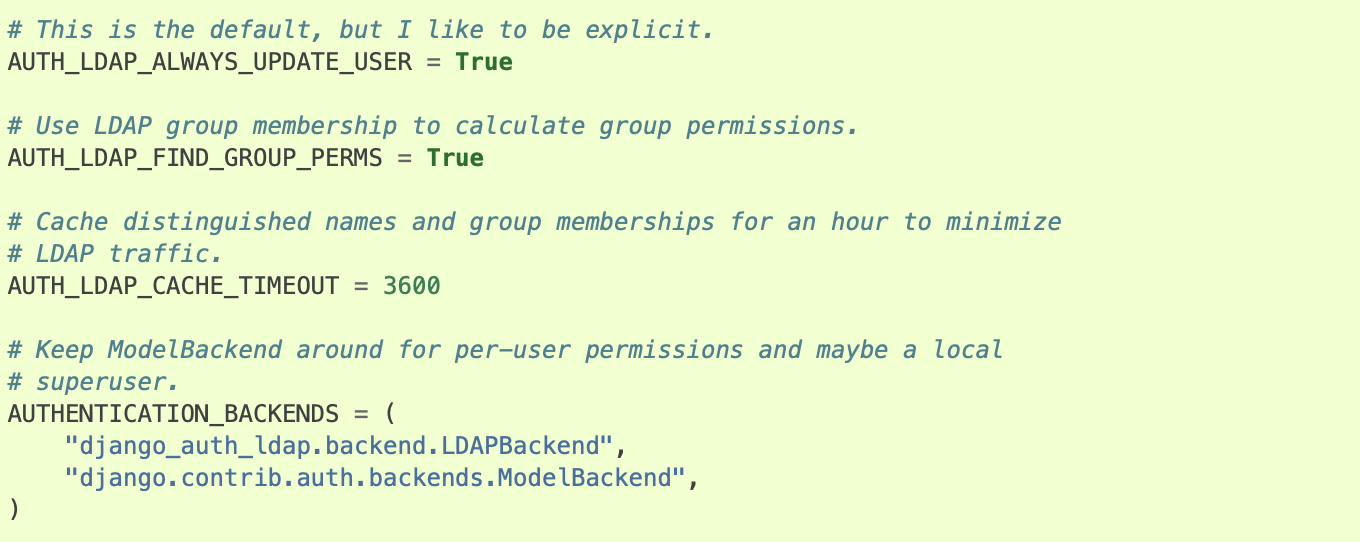
\includegraphics[width=6in]{figures/exam2}
\captionsource{Example Configuration}{\url{https://django-auth-ldap.readthedocs.io/en/latest/example.html}}
\label{figure:exam}
\end{figure}
\newpage

\section{API ที่จะนำมาเรียกใช้}
\cite{restapi}
โดย API ที่จะนำมาเรียกใช้คือ REST API สําหรับการส่งงานเขียนโปรแกรมด้วย OpenAPI และ API ที่ได้พัฒนานี้ จะรับข้อมูลคําตอบได้เฉพาะไฟล์ที่เป็นภาษาคอมพิวเตอร์ แบ่งเป็น 2 รายการดังนี้
\begin{enumerate}
    \item รายการแรกเป็น Compiler API ทําหน้าที่รับข้อมูลจากผู้ใช้และทําการตรวจสอบ
โปรแกรม โดยทําการเปรียบเทียบกับผลเฉลย และส่งผลลัพธ์กลับเป็น output
    \item API รายการที่สองเป็น Problem API สําหรับทําหน้าที่อัปเดตข้อมูลของโจทย์ปัญหาและเฉลย
\end{enumerate}

\subsection{Method ที่เซิร์ฟเวอร์ใช้ในการรับข้อมูลจากผู้ใช้}
ในการพัฒนาระบบ API ได้มีการเลือกใช้ method หลัก ๆ จํานวน 2 method คือ
method GET และ method POST โดยทั้ง 2 method มีความแตกต่างกันดังนี้
\begin{itemize}
    \item GET เป็นการดึงข้อมูลจากฐานข้อมูลของเซิร์ฟเวอร์หรือเว็บไซต์มาแสดงผลออกมาเป็น response
    \item POST เป็นการเพิ่มหรือเปลี่ยนแปลงข้อมูลต่างๆที่อยู่ในฐานข้อมูลของเซิร์ฟเวอร์เว็บไซต์
\end{itemize}
โดย API ทั้ง 2 ตัวได้มีการใช้ method ดังกล่าว ทั้ง 2 ตัวกล่าวคือ ใน Path /compile ได้มีการรองรับ
method GET และ POST และใน Path /problem ก็ได้มีการรองรับ method GET และ POST เช่น
เดียวกัน โดยได้เน้นการทํางานในส่วน method POST ดังนี้
\begin{itemize}
    \item method POST ใน /compile ทําหน้าที่รับข้อมูลเกี่ยวกับงานของนักศึกษาเพื่อนํามาประมวล
ผลและทําการแสดงคะแนนของนักศึกษาคนนั้น ๆ ที่ส่งงานหรือ assignment เข้ามาในระบบ
    \item method POST ใน /problem ทําหน้าที่รอรับ API ของผู้ที่ต้องการตรวจสอบว่า ค่า output
ของ assignment ที่ได้ทําการส่งไป มีคําตอบตรงตามที่เจ้าของ assignment เขียนไว้หรือไม่
\end{itemize}

%% ผลการดำเนินงาน
%% Finding and Results
%%================================================
%% Chapter 4
%%================================================
\chapter{ผลการดำเนินงานและอภิปรายผล}
%\label{result}
\label{chapter4}

\section{หัวข้อใหญ่}

\subsection{หัวข้อย่อยระดับที่ 1}

\subsubsection{หัวข้อย่อยระดับที่ 2}

\section{หัวข้อใหญ่}

\subsection{หัวข้อย่อยระดับที่ 1}

\subsubsection{หัวข้อย่อยระดับที่ 2}



%% สรุปโครงงาน
%% Conclusions and Recommendations
%%================================================
%% Chapter 5
%%================================================
\chapter{สรุปผลการดำเนินงาน อุปสรรค และการพัฒนาในอนาคต}
%\label{conclusion}
\label{chapter5}

\section{สรุปผลโครงงาน}

\subsection{หัวข้อย่อยระดับที่ 1}

\section{ปัญหาและอุปสรรค}

\subsection{หัวข้อย่อยระดับที่ 1}

\section{ข้อเสนอแนะในการพัฒนาต่อ}

\subsection{หัวข้อย่อยระดับที่ 1}


%% ตัวอย่างการเขียน
%% Examples of writing LaTeX
\chapter{ตัวอย่างการเขียน LaTeX}
\label{example}

\section{โครงสร้างของ Template}
ในไฟล์ zip ประกอบด้วยไฟล์ต่าง ๆ ดังต่อไปนี้
\begin{enumerate}[1.]
    \item \filename{thesis.tex} เป็นไฟล์หลักที่ประกอบด้วย ไฟล์ย่อยต่างๆ ตลอดจนข้อมูลของวิทยานิพนธ์ เช่น ชื่อวิทยานิพนธ์ทั้งภาษาไทย และอังกฤษ ชื่อผู้แต่ง ชื่อกรรมการสอบวิทยานิพนธ์
    \item \filename{info.tex} - ไฟล์ที่กำหนดข้อมูลของโครงงาน
    \item \filename{abstract_th.tex} - ไฟล์ที่เขียนบทคัดย่อ ภาษาไทย
    \item \filename{abstract_en.tex} - ไฟล์ที่เขียนบทคัดย่อ ภาษาอังกฤษ
    \item \filename{acronyms.tex} - ไฟล์ที่เขียนสัญลักษณ์ หรือคำย่อ (ถ้าใช้)
    \item \filename{ack_th.tex} - ไฟล์ที่เขียนกิตติกรรมประกาศ ภาษาไทย
    \item \filename{ack_en.tex} - ไฟล์เขียนกิตติกรรมประกาศ ภาษาอังกฤษ (ไม่ใช้ไฟล์นี้)
    \item \filename{chapter[1..5].tex} - ไฟล์ของบทต่าง ๆ ศึกษารายละเอียดของบทต่าง ๆ ในคู่มือวิทยานิพนธ์~\cite{tu:2556fk}
    \item \filename{appendix[A..B].tex} - ไฟล์ภาคผนวก %% โดยภาคผนวกมีได้สูงสุด 10 ภาคผนวก
    \item \filename{refs.bib} - ไฟล์ฐานข้อมูลรายการอ้างอิง (Bibliography) ในรูปแบบ BibTeX
    \item \filename{TUthesis.sty} - ไฟล์ template style สำหรับมหาวิทยาลัยธรรมศาสตร์ (ไม่จำเป็นต้องแก้ไขไฟล์นี้)
    \item \filename{mystyle.sty} - ไฟล์ template style สำหรับปรับแต่งรายงานโครงงาน (ไม่จำเป็นต้องแก้ไขไฟล์นี้)
    \item \filename{example.tex} - ไฟล์ตัวอย่างการเขียน LaTeX
\end{enumerate}

\newpage
\section{การเขียน LaTeX}
สามารถอ่านจากบทความต่าง ๆ
\begin{enumerate}[1.]
    \item บทแนะนำ LaTeX 2e แบบไม่ค่อยย่อ แปลโดย คุณจักรภาษณ์ วิศวกุล\\
    \url{http://zelmanov.ptep-online.com/ctan/lshort_thai.pdf}

    %%\item ตัวอย่างคำสั่ง LaTeX ของภาควิชาคณิตศาสตร์ คณะวิทยาศาสตร์ ม. เชียงใหม่\\
    %% Link down
    %%\url{http://www.math.science.cmu.ac.th/thanasak/pow/CMU_LaTeX_2010_All.pdf} %%
    \item บทแนะนำ LaTeX 2e แบบไม่ค่อยย่อ ภาษาอังกฤษ โดย Tobias Oetiker\\
    \url{https://tobi.oetiker.ch/lshort/lshort.pdf}

    \item ตัวอย่างคำสั่ง LaTeX ของภาควิชาคณิตศาสตร์ คณะวิทยาศาสตร์ ม. เกษตรศาสตร์\\
    \url{http://maths.sci.ku.ac.th/th/service/training/2556/2555-06-17_1/doc_xelatex.pdf}

    \item Thesis template และแนะนำการใช้ LaTeX ของอาจารย์ \mbox{ดร. ฑิตยา หวานวารี}  ภาควิชาคณิตศาสตร์และวิทยาการคอมพิวเตอร์ คณะวิทยาศาสตร์ จุฬาลงกรณ์มหาวิทยาลัย\\
    \url{http://pioneer.netserv.chula.ac.th/~wdittaya/}

    \item LaTeX ใน Wikibook\\
    \url{https://en.wikibooks.org/wiki/LaTeX}

    \item การใช้ Endnote กับ Latex และ BibTeX\\
    \url{http://www.rhizobia.co.nz/latex/convert}
\end{enumerate}

\newpage
\section{การใช้ฟอนต์}
\
ฟอนต์หลักที่ได้กำหนดไว้แล้วในรายงานคือ \texttt{TH Sarabun New} การใช้งานฟอนต์ สามารถเลือกรูปแบบการแสดงได้ดังนี้

\begin{table}[H]
    \centering
    \footnotesize
    \begin{threeparttable}
        \caption{รูปแบบการแสดงฟอนต์}
        \label{tab:font style}
        \begin{tabular}{l c C{6cm} c}
            \toprule
            \textbf{รูปแบบ} & \textbf{คำสั่ง} & \textbf{ตัวอย่างการใช้คำสั่ง} & \textbf{ผลการแสดง} \\
            \midrule
            ตัวหนา & \verb|\textbf{text}| & \verb|\textbf{|พลังของแผ่นดิน\verb|}| & \textbf{พลังของแผ่นดิน} \\
            ตัวเอียง & \verb|\textit{text}| & \verb|\textit{|พลังของแผ่นดิน\verb|}| & \textit{พลังของแผ่นดิน} \\
            ตัวเอียงและหนา & \verb|\textit{\textbf{text}}| & \verb|\textit{\textbf{|พลังของแผ่นดิน\verb|}}| & \textit{\textbf{พลังของแผ่นดิน}} \\
            ตัวหนาและเอียง & \verb|\textbf{\textit{text}}| & \verb|\textbf{\textit{|พลังของแผ่นดิน\verb|}}| & \textbf{\textit{พลังของแผ่นดิน}} \\
            ขีดเส้นใต้ & \verb|\underline{text}| & \verb|\underline{|พลังของแผ่นดิน\verb|}| & \underline{พลังของแผ่นดิน} \\
            ตัวหนาและเอียง\footnotetext[1]{test} & \verb|\underline{\textit{text}}| & \verb|\underline{\textit{|พลังของแผ่นดิน\verb|}}| & \underline{\textit{พลังของแผ่นดิน}} \\
            เน้นข้อความ\tnote{1} & \verb|\emph{text}| & \verb|\emph{|พลังของแผ่นดิน\verb|}| & \emph{พลังของแผ่นดิน} \\
            \bottomrule
        \end{tabular}
        \begin{tablenotes}
            \item [1] ปกติจะแสดงเป็นแบบเดียวกับตัวเอียง (italic)
        \end{tablenotes}
    \end{threeparttable}
\end{table}

LaTeX มีคำสั่งในการเปลี่ยนขนาดฟอนต์ แต่สำหรับในรายงานโครงงาน ไม่จำเป็นต้องเปลี่ยนขนาดฟอนต์ คำสั่งใน \autoref{tab:font size} เหล่านี้จะเปลี่ยนขนาดของฟอนต์ที่ใช้ในสภาพแวดล้อม\mbox{ปัจจุบัน} จนกว่าจะมีการใช้คำสั่งเปลี่ยนขนาดใหม่

\begin{table}[H]
    \centering
    \footnotesize
    \begin{threeparttable}
        \caption{เปลี่ยนขนาดของฟอนต์}
        \label{tab:font size}
        \begin{tabular}{l C{6cm} c}
            \toprule
            \textbf{คำสั่ง} & \textbf{ตัวอย่างการใช้คำสั่ง} & \textbf{ผลการแสดง} \\
            \midrule
            \verb|\tiny| & \verb|\tiny| พลังของแผ่นดิน & \tiny พลังของแผ่นดิน \\
            \verb|\scriptsize| & \verb|\scriptsize|พลังของแผ่นดิน| & \scriptsize พลังของแผ่นดิน \\
            \verb|\footnotesize| & \verb|\footnotesize| พลังของแผ่นดิน & \footnotesize พลังของแผ่นดิน \\
            \verb|\small| & \verb|\small| พลังของแผ่นดิน & \small พลังของแผ่นดิน \\
            \verb|\normalsize| & \verb|\normalsize|พลังของแผ่นดิน & \normalsize พลังของแผ่นดิน \\
            \verb|\large| & \verb|\large| พลังของแผ่นดิน & \large พลังของแผ่นดิน \\
            \verb|\Large| & \verb|\Large| พลังของแผ่นดิน & \Large พลังของแผ่นดิน \\
            \verb|\LARGE| & \verb|\LARGE| พลังของแผ่นดิน & \LARGE พลังของแผ่นดิน \\
            \verb|\huge| & \verb|\huge| พลังของแผ่นดิน & \huge พลังของแผ่นดิน \\
            \verb|\Huge| & \verb|\Huge| พลังของแผ่นดิน & \Huge พลังของแผ่นดิน \\
            \bottomrule
        \end{tabular}
    \end{threeparttable}
\end{table}

ในกรณีที่ต้องการเปลี่ยนขนาดฟอนต์เฉพาะบางส่วนของข้อความ ให้เขียนคำสั่งภายในสภาพแวดล้อมปิด (อยู่ภายในเล็บวงเล็บปีกกา) เช่น \verb|{\footnotesize test}|

\newpage
\section{การเพิ่มรายการ (List)}

รูปแบบคำสั่งในการเขียนรายการใน LaTeX คือ

\begin{lstlisting}[caption={รูปแบบคำสั่งในการเขียนรายการ (list)}, label={list:list format},language=TeX]
\begin{|\textcolor{blue}{list\_type}|}
    \item รายการที่ 1
    \item รายการที่ 2
    \item รายการที่ 3
\end{|\textcolor{blue}{list\_type}|}
\end{lstlisting}

โดย \textcolor{blue}{\texttt{list\_type}} ใน \autoref{list:list format} มีอยู่ 3 แบบคือ

\begin{itemize}[noitemsep]
    \item \textbf{\color{blue}itemize} รายการแบบใช้สัญลักษณ์ (เช่น bullet point)
    \item \textbf{\color{blue}enumerate} รายการแบบใช้ตัวเลข (หรือตัวอักษร เช่น 1. (a))
    \item \textbf{\color{blue}description} รายการแบบการอธิบายคำ
\end{itemize}

%%=================================================
%% Itemize
%%=================================================

\subsection{ตัวอย่างรายการแบบ \textcolor{blue}{itemize}}

\begin{exampleBox}[sidebyside]{รายการแบบ defaut (bullet)}
\begin{lstlisting}[frame=none,language={[LaTeX]TeX}]
\begin{itemize}
    \item รายการที่ 1
    \item รายการที่ 2
    \item รายการที่ 3
\end{itemize}
\end{lstlisting}
\tcblower
\begin{itemize}[noitemsep]
    \item รายการที่ 1
    \item รายการที่ 2
    \item รายการที่ 3
\end{itemize}
\end{exampleBox}


\begin{exampleBox}[sidebyside]{รายการซ้อนกัน (nested list)}
\small
\begin{lstlisting}[frame=none,language={[LaTeX]TeX}]
\begin{itemize}
    \item รายการระดับ 1
    \begin{itemize}
        \item รายการระดับ 2
        \begin{itemize}
            \item รายการระดับ 3
            \begin{itemize}
                \item รายการระดับ 4
            \end{itemize}
        \end{itemize}
    \end{itemize}
\end{itemize}
\end{lstlisting}
\tcblower
\small
\begin{itemize}[noitemsep,leftmargin=*,label=\textbullet]
    \item รายการระดับ 1
    \begin{itemize}
        \item รายการระดับ 2
        \begin{itemize}
            \item รายการระดับ 3
            \begin{itemize}
                \item รายการระดับ 4
            \end{itemize}
        \end{itemize}
    \end{itemize}
\end{itemize}
\end{exampleBox}


\begin{exampleBox}[lefthand ratio=0.55,sidebyside]{เปลี่ยนสัญลักษณ์ที่ระดับต่าง ๆ}
\small
\begin{lstlisting}[frame=none,language={[LaTeX]TeX}]
\begin{itemize}[\textbullet]
    \item รายการระดับ 1
    \begin{itemize}[\textendash]
        \item รายการระดับ 2
        \begin{itemize}[$\ast$]
            \item รายการระดับ 3
            \begin{itemize}[$\square$]
                \item รายการระดับ 4
            \end{itemize}
        \end{itemize}
    \end{itemize}
\end{itemize}
\end{lstlisting}
\tcblower
\small
\begin{itemize}[\textbullet,noitemsep,leftmargin=*,]
    \item รายการระดับ 1
    \begin{itemize}[\textendash]
        \item รายการระดับ 2
        \begin{itemize}[$\ast$]
            \item รายการระดับ 3
            \begin{itemize}[$\square$]
                \item รายการระดับ 4
            \end{itemize}
        \end{itemize}
    \end{itemize}
\end{itemize}
\end{exampleBox}

%%=================================================
%% Enumerate
%%=================================================

\subsection{ตัวอย่างรายการแบบ \textcolor{blue}{enumerate}}

\begin{exampleBox}[sidebyside]{รายการมีลำดับแบบ defaut (ลำดับเป็นตัวเลขอารบิก)}
\begin{lstlisting}[frame=none,language={[LaTeX]TeX}]
\begin{enumerate}
    \item รายการที่ 1
    \item รายการที่ 2
    \item รายการที่ 3
\end{enumerate}
\end{lstlisting}
\tcblower
\begin{enumerate}[noitemsep]
    \item รายการที่ 1
    \item รายการที่ 2
    \item รายการที่ 3
\end{enumerate}
\end{exampleBox}

\begin{exampleBox}[sidebyside]{รายการซ้อนกัน (nested list)}
\small
\begin{lstlisting}[frame=none,language={[LaTeX]TeX}]
\begin{enumerate}
    \item รายการระดับ 1
    \begin{enumerate}
        \item รายการระดับ 2
        \begin{enumerate}
            \item รายการระดับ 3
            \begin{enumerate}
                \item รายการระดับ 4
            \end{enumerate}
        \end{enumerate}
    \end{enumerate}
\end{enumerate}
\end{lstlisting}
\tcblower
\small
\begin{enumerate}
    \item รายการระดับ 1
    \begin{enumerate}
        \item รายการระดับ 2
        \begin{enumerate}
            \item รายการระดับ 3
            \begin{enumerate}
                \item รายการระดับ 4
            \end{enumerate}
        \end{enumerate}
    \end{enumerate}
\end{enumerate}
\end{exampleBox}

\begin{exampleBox}[sidebyside]{เปลี่ยนหมายเลขลำดับที่ระดับต่าง ๆ}
\small
\begin{lstlisting}[frame=none,language={[LaTeX]TeX}]
\begin{enumerate}[1.]
    \item รายการระดับ 1
    \item รายการระดับ 1
    \item รายการระดับ 1
    \begin{enumerate}[(a)]
        \item รายการระดับ 2
        \item รายการระดับ 2
        \item รายการระดับ 2
        \begin{enumerate}[A)]
            \item รายการระดับ 3
            \item รายการระดับ 3
            \item รายการระดับ 3
            \begin{enumerate}[i.]
                \item รายการระดับ 4
                \item รายการระดับ 4
                \item รายการระดับ 4
            \end{enumerate}
        \end{enumerate}
    \end{enumerate}
\end{enumerate}
\end{lstlisting}
\tcblower
\small
\begin{enumerate}[1.]
    \item รายการระดับ 1
    \item รายการระดับ 1
    \item รายการระดับ 1
    \begin{enumerate}[(a)]
        \item รายการระดับ 2
        \item รายการระดับ 2
        \item รายการระดับ 2
        \begin{enumerate}[A)]
            \item รายการระดับ 3
            \item รายการระดับ 3
            \item รายการระดับ 3
            \begin{enumerate}[i.]
                \item รายการระดับ 4
                \item รายการระดับ 4
                \item รายการระดับ 4
            \end{enumerate}
        \end{enumerate}
    \end{enumerate}
\end{enumerate}
\end{exampleBox}


\begin{exampleBox}[lefthand ratio=0.55,sidebyside]{เปลี่ยนหมายเลขลำดับที่ระดับต่าง ๆ โดยใช้หมายเลขหัวข้อ}
\scriptsize
\begin{lstlisting}[frame=none,language={[LaTeX]TeX}]
\begin{enumerate}[\thesection.\arabic*]
    \item รายการระดับ 1
    \item รายการระดับ 1
    \item รายการระดับ 1
    \begin{enumerate}[\theenumi.\arabic*]
        \item รายการระดับ 2
        \item รายการระดับ 2
        \item รายการระดับ 2
        \begin{enumerate}[\theenumii.\arabic*]
            \item รายการระดับ 3
            \item รายการระดับ 3
            \item รายการระดับ 3
            \begin{enumerate}[\theenumiii.\arabic*]
                \item รายการระดับ 4
                \item รายการระดับ 4
                \item รายการระดับ 4
            \end{enumerate}
        \end{enumerate}
    \end{enumerate}
\end{enumerate}
\end{lstlisting}
\tcblower
\scriptsize
\begin{enumerate}[\thesection.\arabic*]
    \item รายการระดับ 1
    \item รายการระดับ 1
    \item รายการระดับ 1
    \begin{enumerate}[\theenumi.\arabic*]
        \item รายการระดับ 2
        \item รายการระดับ 2
        \item รายการระดับ 2
        \begin{enumerate}[\theenumii.\arabic*]
            \item รายการระดับ 3
            \item รายการระดับ 3
            \item รายการระดับ 3
            \begin{enumerate}[\theenumiii.\arabic*]
                \item รายการระดับ 4
                \item รายการระดับ 4
                \item รายการระดับ 4
            \end{enumerate}
        \end{enumerate}
    \end{enumerate}
\end{enumerate}
\end{exampleBox}
\newpage
\section{การเพิ่มรูป}

\begin{exampleBox}[lefthand ratio=0.7,sidebyside]{เพิ่มรูปโดยใช้สภาพแวดล้อม \texttt{figure}}
\footnotesize
\begin{lstlisting}[frame=none]
\begin{figure}[H]
    \centering
    
\includegraphics[width=2cm]{figures/tu-logo-bw.jpg}
    \caption{ตราธรรมจักร}
    \label{fig:thammajak}
\end{figure}
\end{lstlisting}
\tcblower
\footnotesize
\begin{figure}[H]
    \centering
    
\includegraphics[width=2cm]{figures/tu-logo-bw.jpg}
    \caption{ตราธรรมจักร}
    \label{fig:thammajak}
\end{figure}
\end{exampleBox}

การเขียนคำอธิบายรูป ในกรณีที่เป็นรูปที่สร้างขึ้นเอง ไม่จำเป็นต้องระบุแหล่งที่มา ให้ใช้คำสั่ง \latex{\caption{figure description}} เช่น ใน \autoref{fig:thammajak} ให้ใช้คำสั่ง \verb|\caption{|ตราธรรมจักร\verb|}|

วิธีการอ้างอิงถึงรูป ให้ใช้คำสั่ง \latex{\ref{label}} หรือ \latex{\autoref{label}} เช่น หากต้องการอ้างอิงถึง \autoref{fig:thammajak} ข้างต้น ให้พิมพ์ รูปที่ \latex{\ref{fig:thammajak}} หรือ \latex{\autoref{fig:thammajak}}


\begin{figure}[H]
    \centering
    
\includegraphics[width=2cm]{figures/tu-logo-bw.jpg}
    \captionsource{ตราธรรมจักร}{\url{https://tu.ac.th/thammasat-identity}}
    \label{fig:thammajak 2}
\end{figure}

แต่ถ้าได้รูปมาจากที่อื่น ให้ระบุแหล่งที่มาด้วย โดยให้ใช้คำสั่ง \latex{\captionsource{figure description}{figure source}} เช่น หากต้องการระบุแหล่งที่มาใน \autoref{fig:thammajak 2} ให้พิมพ์คำสั่ง \\ \verb|\captionsource{|ตราธรรมจักร\verb|}{\url{https://tu.ac.th/thammasat-identity}}|

\begin{exampleBox}{แสดงหลายรูปย่อยโดยใช้สภาพแวดล้อม \texttt{subfigure}}
\footnotesize
\begin{lstlisting}[frame=none]
\begin{figure}[H]
    \centering
    \begin{subfigure}[b]{0.45\textwidth}
        \centering
        
\includegraphics[width=1.5in]{tu-logo-bw}
        \caption{|ตราธรรมจักร ขาวดำ|}
        \label{fig:thammajak bw}
    \end{subfigure}
    ~ %add desired spacing between images, e. g. ~, \quad, \qquad, \hfill etc.
      %(or a blank line to force the subfigure onto a new line)
    \begin{subfigure}[b]{0.45\textwidth}
        \centering
        
\includegraphics[width=1.5in]{tu-logo-color}
        \caption{|ตราธรรมจักร สี|}
        \label{fig:thammajak color}
    \end{subfigure}
    \caption{|ตราธรรมจักร ขาวดำและสี|}\label{fig:thammajak both color}
\end{figure}
\end{lstlisting}
\tcblower
\footnotesize
\begin{figure}[H]
    \centering
    \begin{subfigure}[b]{0.45\textwidth}
        \centering
        
\includegraphics[width=1.5in]{tu-logo-bw}
        \caption{ตราธรรมจักร ขาวดำ}
        \label{fig:thammajak bw}
    \end{subfigure}
    ~ %add desired spacing between images, e. g. ~, \quad, \qquad, \hfill etc.
    %(or a blank line to force the subfigure onto a new line)
    \begin{subfigure}[b]{0.45\textwidth}
        \centering
        
\includegraphics[width=1.5in]{tu-logo-color}
        \caption{ตราธรรมจักร สี}
        \label{fig:thammajak color}
    \end{subfigure}
    \caption{ตราธรรมจักร ขาวดำและสี}\label{fig:thammajak both color}
\end{figure}
\end{exampleBox}


\newpage
\section{การเพิ่มตาราง}

\begin{exampleBox}{เพิ่มตาราง ใช้เส้นขอบขั้น}
\begin{lstlisting}[frame=none,escapeinside={!}{!}]
\begin{table}[H]
    \centering
    \caption{!ตัวอย่างตาราง!}
    \label{tab:table 1}
    \begin{tabular}{| c | c | p{3cm} | p{3cm} |}
        \hline
        !หัวตาราง 1! & !หัวตาราง 1! & !หัวตาราง 1! & !หัวตาราง 1! \\
        \hline
        ข้อมูล & ข้อมูล & ข้อมูล & ข้อมูล \\
        \hline
        ข้อมูล & ข้อมูล & ข้อมูล & ข้อมูล \\
        \hline
        ข้อมูล & ข้อมูล & ข้อมูล & ข้อมูล \\
        \hline
    \end{tabular}
\end{table}
\end{lstlisting}
\tcblower
\begin{table}[H]
    \centering
    \caption{ตัวอย่างตาราง}
    \label{tab:table 1}
    \begin{tabular}{| c | c | p{3cm} | p{3cm} |}
        \hline
        หัวตาราง 1 & หัวตาราง 1 & หัวตาราง 1 & หัวตาราง 1 \\
        \hline
        ข้อมูล & ข้อมูล & ข้อมูล & ข้อมูล \\
        \hline
        ข้อมูล & ข้อมูล & ข้อมูล & ข้อมูล \\
        \hline
        ข้อมูล & ข้อมูล & ข้อมูล & ข้อมูล \\
        \hline
    \end{tabular}
\end{table}
\end{exampleBox}

\newpage
\begin{exampleBox}{เพิ่มตาราง}
\begin{lstlisting}[frame=none]
\begin{table}
    \centering
    \caption{|ตัวอย่างตาราง|}
    \label{tab:table 2}
    \begin{tabular}{c c p{3cm} p{3cm}}
        \toprule
        |หัวตาราง 1| & |หัวตาราง 1| & |หัวตาราง 1| & |หัวตาราง 1| \\
        \midrule
        ข้อมูล & ข้อมูล & ข้อมูล & ข้อมูล \\
        ข้อมูล & ข้อมูล & ข้อมูล & ข้อมูล \\
        ข้อมูล & ข้อมูล & ข้อมูล & ข้อมูล \\
        \bottomrule
    \end{tabular}
\end{table}
\end{lstlisting}
\tcblower
\begin{table}[H]
    \centering
    \caption{ตัวอย่างตาราง ไม่มีเส้นขอบขั้น}
    \label{tab:table 2}
    \begin{tabular}{c c p{3cm} p{3cm}}
        \toprule
        หัวตาราง 1 & หัวตาราง 1 & หัวตาราง 1 & หัวตาราง 1 \\
        \midrule
        ข้อมูล & ข้อมูล & ข้อมูล & ข้อมูล \\
        ข้อมูล & ข้อมูล & ข้อมูล & ข้อมูล \\
        ข้อมูล & ข้อมูล & ข้อมูล & ข้อมูล \\
        \bottomrule
    \end{tabular}
\end{table}
\end{exampleBox}

\newpage
\section{การอ้างอิง (รายการอ้างอิง)}
รูปแบบที่ตั้งไว้ใน template นี้ โดยคำสั่งที่กำหนดไว้ ใน \filename{mystyle.sty} คือ
\begin{enumerate}
    \item \latex{\usepackage[backend=biber,style=ieee,bibencoding=utf8]{biblatex}}
    \item \latex{\addbibresource{refs.bib}} โดย \filename{refs.bib} คือไฟล์ฐานข้อมูลรายการอ้างอิงในรูปแบบ BibTeX
    \item เวลาอ้างอิง ให้ใช้คำสั่ง \latex{\cite{key}}
\end{enumerate}

\subsection{ตัวอย่างการอ้างอิง}

\subsubsection{การอ้างอิงหนังสือ}

ให้เขียนข้อมูลรายการของหนังสือที่ต้องการอ้างอิง เก็บไว้ในไฟล์ \filename{refs.bib} ตัวอย่างเช่น \autoref{list:ref book}

\begin{lstlisting}[caption={ตัวอย่างการอ้างอิงหนังสือ},label={list:ref book}]
@book{Oversampling:1992,
    editor        = "J. C. Candy and G. C. Temes",
    title         = "Oversampling Delta-Sigma Data Converters Theory,
                     Design and Simulation",
    publisher     = "{IEEE} Press.",
    location      = "New York",
    year          = "1992"
}
\end{lstlisting}

ชื่อที่ต้องใช้ในการอ้างอิงสำหรับ \autoref{list:ref book} คือ \latex{Oversampling:1992} โดยเราสามารถ\mbox{กำหนด}ชื่อนี้ได้เอง การอ้างอิงใน \autoref{list:ref book} ให้ใช้คำสั่ง \latex{\cite{Oversampling:1992}} \cite{Oversampling:1992}


\begin{lstlisting}[caption={ตัวอย่างการอ้างอิงบทความ},label={list:ref article}]
@article{Midgap:1997,
    author        = "A. Castaldini and A. Cavallini and B. Fraboni
                     and P. Fernandez and J. Piqueras",
    title         = "Midgap Traps Related to Compensation Processes in
                     {CdTe} Alloys",
    journaltitle  = "Phys. Rev. B.",
    volume        = "56",
    number        = "23",
    year          = "1997",
    pages         = "14897-14900"
}
\end{lstlisting}

สำหรับข้อมูลใน \autoref{list:ref article} ชื่อที่จะใช้ในการอ้างอิงคือ \latex{Midgap:1997} โดยการ\mbox{อ้างอิง} ให้ใช้คำสั่ง \latex{\cite{Midgap:1997}} \cite{Midgap:1997}

\subsubsection{การอ้างอิงเอกสารออนไลน์}

\begin{lstlisting}[caption={ตัวอย่างการอ้างอิงเอกสารออนไลน์ 1},label={list:ref online 1}]
@misc{NFC,
author        = "|{เสฏฐวุฒิ แสนนาม}|",
title         = "{NFC}",
year          = "2013",
howpublished  = "|\url{https://www.thaicert.or.th/papers/general/2013/pa2013ge001.html}|",
}
\end{lstlisting}

การอ้างอิงใน \autoref{list:ref online 1} ให้ใช้คำสั่ง \latex{\cite{NFC}} \cite{NFC}




%%=================================================
%% References
%%=================================================
%%=================================================
%% References
%%=================================================
%% \bibliography refers to your BibTeX .bib file, e.g. refs.bib
\backmatter
\cleardoublepage  %% needed to ensure TOC page number is correct
\phantomsection
\raggedright
\renewcommand{\bibname}{รายการอ้างอิง}
%\renewcommand{\bibname}{บรรณานุกรม}

\addtocontents{toc}{\protect\vspace{\baselineskip}}
\addcontentsline{toc}{chapter}{\bibname}
\addtocontents{toc}{\protect\vspace{\baselineskip}}

%{หนังสือและบทความในหนังสือ}
%\printbibliography[type=book]

%{บทความวารสาร}
%{บทความหนังสือพิมพ์}
%\printbibliography[type=article]

%{วิทยานิพนธ์}
%\printbibliography[type=phdthesis]
%\printbibliography[type=masterthesis]

%{สื่ออิเล็กทรอนิกส์}
%\printbibliography[type=misc]

%% no categories for now
\printbibliography



%%=================================================
%% Appendices
%%=================================================
%% Edit the files appendixA.tex, appendixB.tex, ...
%% If you have more appendices, add appendC, appendD, ...
\IfAddAppendix{
	\appendix
	\appendixpage
	%%================================================
%% Appendix A
%%================================================
\chapter{ตัวอย่างภาคผนวก}
\label{appA}

This is an example appendix. This is an example appendix. This is an example appendix. This is an example appendix. This is an example appendix. This is an example appendix. This is an example appendix. This is an example appendix. This is an example appendix. This is an example appendix.


	%%================================================
%% Appendix B
%%================================================
\chapter{Example Appendix}
\label{appB}

This is an example appendix. This is an example appendix. This is an example appendix. This is an example appendix. This is an example appendix. This is an example appendix. This is an example appendix. This is an example appendix. This is an example appendix. This is an example appendix.


}

\end{document}
